\documentclass[12pt]{article}
%\usepackage{fontspec}
 
%\setmainfont{Times New Roman}

\usepackage{newtxtext,newtxmath}


\usepackage[vmargin=1in,hmargin=1in]{geometry}
\usepackage{amsmath}
\usepackage[parfill]{parskip}
\usepackage{hyperref}
\usepackage{natbib}
\usepackage{bm}
\usepackage{amsfonts}
\usepackage{graphicx}
\usepackage{abstract}
\usepackage{lineno}
\usepackage{setspace,caption}
\captionsetup{font=doublespacing}% Double-spaced float captions


\bibliographystyle{ecology}
\setlength{\bibsep}{0pt}


\hypersetup{pdfstartview={Fit},hidelinks}

\setlength{\absleftindent}{0pt}
\setlength{\absrightindent}{0pt}

\newcommand{\bs}{{\bf s}}
\newcommand{\bsi}{{\bf s}_i}
\newcommand{\bx}{{\bf x}}
\newcommand{\bxj}{{\bf x}_j}
\newcommand{\by}{{\bf y}}
\newcommand{\bu}{{\bf u}}
\newcommand{\bui}{{\bf u}_i}
\newcommand{\but}{{\bf u}_{t}}
\newcommand{\buit}{{\bf u}_{it}}
\newcommand{\ed}{\|\bx - \bx'\|}
\newcommand{\cS}{\mathcal{S} }




\begin{document}


\title{Modeling abundance, distribution, movement, and space
  use with camera and telemetry data}
\author{Richard B. Chandler$^1$\footnote{Corresponding author: rchandler@warnell.uga.edu}, Daniel A. Crawford$^2$, Elina P. Garrison$^3$, \\
  Karl V. Miller$^1$, Michael J. Cherry$^2$}

\maketitle

\vspace{12pt}

\begin{description}%[labelindent=1pt]%[leftmargin=1cm]%,labelwidth=\widthof{\bfseries Example:}]
%  \large
\item[$^1$] Warnell School of Forestry and Natural Resources, University of Georgia %\\
\item[$^2$] Caesar Kleberg Wildlife Research Institute at Texas A\&M University-Kingsville %\\
\item[$^3$] Florida Fish and Wildlife Conservation Commission %\\
\end{description}


\vspace{24pt}

Open Research: Data and code are publicly available at
\url{https://github.com/rbchan/scr-move}. The current state of the
repository is attached as a zip file.  

Running Head: Inference from camera and telemetry data


\clearpage


\linenumbers
\doublespacing


\begin{abstract}
\noindent \normalsize
Studies of animal abundance and distribution are often conducted
independently of research on movement, despite the important links
between processes. Movement can cause rapid changes in spatial
variation in density, and movement influences detection probability
and hence estimates of abundance from inferential methods such as
spatial capture-recapture (SCR). Technological developments including
camera traps and GPS telemetry have opened new opportunities for
studying animal demography and movement, yet statistical models for
these two data types have largely developed along parallel tracks. We
present a hierarchical model in which both datasets are conditioned on
a movement process for a clearly-defined population. We fit the model
to data from 60 camera traps and 23,572 GPS telemetry locations
collected on 17 male white-tailed deer in the Big Cypress National
Preserve, Florida, USA during July 2015. Telemetry data were collected
on a 3-4 hr acquisition schedule, and we modeled the movement paths of
all individuals in the region with a Ornstein-Uhlenbeck process that
included individual-specific random effects. Two of the 17 deer with
GPS collars were detected on cameras. An additional 20 male deer
without collars were detected on cameras and individually identified
based on their unique antler characteristics. Abundance was 126 (95\%
CI: 88--177) in the 228 km$^2$ region---only slightly higher than
estimated by a standard SCR model: 119 (84--168). The standard SCR
model, however, was unable to describe individual heterogeneity in
movement rates and space use as revealed by the joint model. Joint
modeling allowed the telemetry data to inform the movement model and
the SCR encounter model, while leveraging information in the camera
data to inform abundance, distribution, and movement. Unlike most
existing methods for population-level inference on movement, the joint
SCR-movement model can yield unbiased inferences even if non-uniform
sampling is used to deploy transmitters. Potential extensions of the
model include the addition of resource selection parameters, and
relaxation of the closure assumption when interest lies in survival
and recruitment. These developments would contribute to the emerging
holistic framework for the study of animal ecology---one that uses
modern technology and spatio-temporal statistics to learn about
interactions between behavior and demography. 
%\end{onecolabstract}
\end{abstract}

  
%\vspace{12pt}
\noindent
Keywords: Home range, Ornstein-Uhlenbeck bridge, spatial population
dynamics, spatio-temporal models, utilization distributions



\clearpage

\section{Introduction}

A fundamental challenge facing the study of animal populations is
that the processes governing abundance and distribution -- 
survival, reproduction, and movement -- are highly interwoven and
difficult to directly observe
\citep{williams_etal:2002,royle_dorazio:2008}. Consequently, many
studies of species distributions ignore demographic processes, and
instead model spatial variation in abundance or occurrence as a
function of abiotic variables \citep{elith_etal:2006}. However, even
for studies occurring over short time periods when it is reasonable
to ignore changes resulting from mortality and reproduction, movement
can exert strong influence on the spatial distribution of individuals
\citep{jouventin_weimerskirch:1990,andrew_fox:2020}.
The importance of accounting for animal movement in studies of
abundance and distribution is gaining recognition, but few statistical
frameworks exist for joint inference
\citep{morales_etal:2010,matthiopoulos_etal:2015,spiegel_etal:2017}. 

The ability to observe population processes has improved in
recent years as a result of new data collection technologies. 
GPS telemetry has ushered in a new era of research
on animal movement, and camera traps have made it possible to 
study the abundance and distribution of even the most elusive species
\citep{cagnacci_etal:2010,oconnell_etal:2010}. Following closely
behind the technological developments have been novel statistical
models allowing for insights about distribution and movement from data
subject to observation error
\citep{royle_etal:2014,hooten_etal:2017}. 
However, the development of movement models for telemetry data, and
the development of distribution models for camera data
have largely proceeded along parallel tracks, limiting the scope of
inferences \citep{mcclintock_etal:2021}. 

Spatial capture-recapture (SCR) methods are widely used with camera
data to study animal abundance and distribution. When animals can be
individually recognized, the location and frequency
of detection events provide information about encounter rates, which
are needed to infer the abundance and distribution of individuals not
detected \citep{efford:2004,borchers_efford:2008,royle_etal:2014}.  
These methods were intentionally developed without
explicit movement processes because modeling movement was not the
motivating objective, recapture rates are often low, and adding
movement into SCR models involves substantial computational challenges
\citep{borchers:2012,borchers_etal:2014}. Emphasis has
therefore been on simple detection functions based on the distance
between activity centers (i.e., the average location of an individual
during the sampling period) and traps. Most SCR observation models
imply that space usage is proportional to an isotropic bivariate normal
distribution, and no serial correlation exists in detection events
\citep[but see][for models implying anisotropic home ranges]{royle_etal:2013,royle_etal:2013mee,royle_etal:2016,chandler_etal:2018mee}.

Movement models for telemetry data have proliferated in recent years
in response to several factors, including technological developments,
growing interest in behavioral responses to
environmental heterogeneity, questions about energetics and space use
in novel environments, and the desire to understand how habitat
selection decisions affect spatial population dynamics  
\citep{lima_zollner:1996,turchin:1998,gaillard_etal:2010,clobert_etal:2012,hooten_etal:2019}.
A concern with many movement models used for population-level
inference is that telemetry datasets are often comprised of a small 
sample of individuals that may not be representative of the population 
\citep{fieberg_etal:2010,hanks_etal:2011,fleming_etal:2019}.
In the absence of known inclusion probabilities
(e.g., constant capture probabilities induced by random sampling),
drawing inferences from a non-uniform sample to the population
requires additional information, such as capture-recapture data to
estimate the parameters of an observation model describing how
individuals enter the sample  
\citep{tufto_etal:2012,gurarie_ovaskainen:2013,pedersen_weng:2013,raabe_etal:2014,mcclintock_etal:2021}.

The limitations associated with independent analyses of
capture-recapture and telemetry datasets in studies of 
abundance, distribution, space use and movement have been recognized
for many years \citep[pp. 534--535]{royle_etal:2014}.
Jointly analyzing both sources of data by embedding a movement process
in an SCR model should allow for improved population-level inference
on movement while providing a more mechanistic description of the
detection process that is key to understanding abundance and
distribution. We present an integrated model for camera and telemetry
data  collected on white-tailed deer  ({\it Odocoileus virginianus}) in
Big Cypress National Preserve, USA where deer are the primary prey of
the endangered Florida panther ({\it Puma concolor coryi}). 
The objective of the research was to understand the effects of panther
predation and changes in hydrology and hunting regulations on deer
populations, but here we use the data as a case study to evaluate the
costs and benefits of embedding a movement process in spatial
capture-recapture models. 


\section{Methods}

\subsection{Model}

\subsubsection{Abundance and distribution}

As with standard SCR models, a point process is used for the 
abundance and distribution of activity centers: $\bs_1, \dots, \bs_N$
in the spatial region $\mathcal{M} \subset \mathbb{R}^2$
(Table~\ref{tab:defs}). Depending on the species, activity centers
over the course of the survey might correspond to territory centers or 
home range centers. Both $N$ and $\bs_1, \dots, \bs_N$ are
stochastic outcomes whose expected values are determined by an
intensity function, $\lambda(\bs)$, describing the distribution of
individuals in terms of spatial variation in the density of activity
centers. The expected value of abundance is given by  the volume under
this surface $E(N) = \Lambda = \int_{\mathcal{M}} \lambda(\bs) \, d\bs$.
The density surface can be modeled as a function of spatial covariates
or spatial random effects. The realized value of abundance is
typically assumed to be $N \sim \mathrm{Pois}(\Lambda)$, although a
binomial distribution is commonly used in Bayesian analyses involving
data augmentation, as described in Sec.~\ref{ssec:n0}. 


\subsubsection{Movement}

Unlike standard SCR models in which the encounter history data are
modeled as a function of the distance between activity centers and
traps, we impose a movement model, and assume that the encounter
histories depend on the time-varying distance between individuals and
traps. Although any movement model could be used in principle, we
adopt the Ornstein-Uhlenbeck (OU) process as it aligns well with SCR
models in that it assumes each animal has its own activity center
around which movement is concentrated. However, unlike most SCR
models, the OU model describes serial correlation in animal locations
($\{{\bm \mu}_{it}\}$ for $i=1,\dots,N$ and $t=1,\dots,T$), and hence in
detection events. For simplicity, we assume no measurement error in
telemetry data ($\{\buit\}$), such that the observed 
location is identical to the actual location $\buit \equiv {\bm
  \mu}_{it}$. In continuous time, the OU process can be written as
a stochastic differential equation or as a bivariate Gaussian process:
\begin{equation}
  p(\bu_{i,t+h}|\buit,\bsi) = \mathrm{Norm}(\bsi + e^{{\bf B}h}(\buit-\bsi), \bm{\Sigma} - e^{{\bf B} h} {\bm \Sigma} e^{\bf{B}' h})
  \label{eq:ou-ct}
\end{equation}
where $\buit$ is the location of individual $i$ at time $t$, $h$ is
a time interval, $e$ is the matrix exponential, and $\bf B$ and $\bm
\Sigma$ are $2\times 2$ matrices 
\citep{dunn_gipson:1977,blackwell:1997,blackwell_etal:2016}.
A simplified, discrete-time version of Eq.~\ref{eq:ou-ct} can be
derived by setting $h=1$ and assuming no covariance between the two
position coordinates, such that ${\bf B} = \rho \mathbf{I}$ and
${\bm \Sigma} = \sigma^2\mathbf{I}$. 
This formulation of the OU model is similar to a biased random walk, 
with the parameters $\rho$ and $\sigma$ determining serial
correlation between locations (Fig.~\ref{fig:ou-concept}). Note that
if $\rho=0$, then the locations would be independent outcomes of
a bivariate normal distribution with mean $\bsi$ and variance $\bm
\Sigma$. At the other extreme, if $\rho=1$, then the variance would
be 0 and the locations would be perfectly correlated (i.e, there would
be no movement). Variation in the parameters can be modeled as functions of 
covariates or as individual-specific random effects as we demonstrate
in the case study.


\subsubsection{Space use and utilization distributions}

The proposed modeling framework allows for inference on space use at
multiple time scales. For example, the area used during the sampling
period can be computed from the posterior distribution of the movement
path. The approach can be viewed as an extension of Brownian bridge
estimators \citep{horne_etal:2007}, with the difference being that an
OU bridge, influenced by the activity center, is used to describe
uncertainty about the movement path between observed telemetry
locations. The probability distributions of these bridges describe
the utilization distribution (UD) for the sampling period. 
Space use can be computed for various quantiles of
the UD, for example to assess the size of 50\% core areas. 
In practice, the utilization distribution can be approximated by
applying a spatial histogram estimator or a kernel density estimator
to posterior samples of the movement path. 

In some settings, interest may be on the area that could have
been used by an animal during a longer time period \citep{fleming_etal:2015}.
Addressing this question requires switching emphasis from the
realized movement path to the expected distribution of locations as
predicted by the fitted model. The distribution of expected locations
over an infinite time horizon is known as the limiting distribution,
which for an OU model is stationary:
\begin{equation}
  p(\bui) = \lim\limits_{h \to \infty} p(\bu_{i,t+h}|\buit,\bsi) = \mathrm{Norm}(\bsi, \bm{\Sigma}).
  \label{eq:ud}
\end{equation}
As with time-specific utilization distributions, the area of the
stationary UD can be computed from isopleths corresponding to
quantiles of interest.
Variation in home range size among individuals can be modeled through
variation in the parameters ($\rho$ and $\sigma$) of the movement model.


\subsubsection{Camera and telemetry data}

We make the standard mark-recapture assumption that the focal species
can be identified to individual when captured. In the case of
camera data, this means that the species has unique natural
markings, making it possible to recognize individuals detected in
photographs and thereby create spatial encounter histories. Let
$y_{ijt}$ indicate either the binary detection event or the frequency
of detections of individual $i\in 1,\dots,n^{\mathrm det}$ at camera
location $j \in 1,\dots,J$ on occasion $t\in 1,\dots,T$, where
$n^{\mathrm det}$ is the number of individuals detected out of
the $N$ individuals in the 
region $\mathcal{M}$. Note that, unlike telemetry data which
correspond to locations at instances in time, the $T$ occasions in
the encounter histories are time {intervals} spanning $(t,t+1)$.

The expected frequency of detections is modeled as a function of
the Euclidean distance between traps and animal locations:
\begin{equation}
  \lambda^{\rm det}_{ijt} = g_0\exp(-\|\bx_{j}-\buit\|^2)/(2\sigma_{\rm det}^2)
  \label{eq:p}
\end{equation}
where $g_0$ is the baseline encounter rate when the distance between
a trap at location $\bx_j$ and an individual at location
$\buit$ is zero. The parameter $g_0$ describes the expected number of 
detections during the interval, conditional on the individual's
location at the beginning of the interval.
The scale parameter $\sigma_{\rm det}^2$ determines
the rate at which detection probability decreases with distance. This is a
localized version of the standard SCR encounter function.

If telemetry data were available for all $N$ individuals in the
region, and the acquisition schedule was set to regular intervals for
all occasions, the locations and hence the distances in Eq.~\ref{eq:p}
would be known. However, when $n^{\mathrm det}<N$ as is always the case, the
locations of the undetected individuals must be inferred. Moreover,
even for the individuals with transmitters, telemetry locations will often
be missing, either because the temporal resolution of interest is
finer than the acquisition interval, or because of transmission
failures. Given that detection probability depends on these unobserved
locations, they must be either estimated or marginalized out of the posterior
distribution during model fitting (see Sec.~\ref{ssec:n0}).

\subsubsection{Transmitter deployment process}
\label{ssec:tr-deploy}

Thus far, we have implicitly assumed that all 
individuals with transmitters have at least one detection in the encounter history
array in $\bm y$. This assumption is required by standard mark-recapture
methods, which effectively estimate the number of individuals not
detected. %, $n_0 = N-n$.
However, this assumption will be violated if
the process used to deploy transmitters is different than the process
used to detect individuals because some individuals with transmitters
will have no detections in the encounter history data. For example, if
transmitters are deployed on individuals captured via live-trapping,
but the encounter histories are generated from camera data, some of
the animals with transmitters may not be detected on the cameras,
resulting in ``all zero'' encounter histories, which are assumed to be
unobservable by most estimation methods \citep{williams_etal:2002}. To
properly describe the data generating process and obtain
valid inference, a model is needed to describe how some, but not all,
of the ``all zero'' encounter histories arise in the encounter
histories. 

One approach for accommodating individuals that were never detected by
cameras, while conditioning on their telemetry data and using it to
estimate encounter rate parameters and abundance, is to model the
transmitter deployment process. The deployment process
can vary widely among taxa, but it usually involves live capture
and therefore can result in a type of mark-recapture
data. For simplicity, assume that the spatial region $\mathcal{M}$ is
uniformly searched, and the $N$ individuals are subject to capture on
a single occasion with probability $p^{\rm cap}$. Let $n^{\rm cap}$ indicate
the number of individuals captured and fitted with
transmitters. Although there may be no recapture data, 
the addition of the new parameter $p^{\rm cap}$ provide a mechanism
for describing how individuals not detected by cameras appear in
the camera-based encounter histories. Specifically, 
we add the model component: 
$y^{\rm cap}_i \sim \mathrm{Bern}(p^{\rm cap})$ for the data from the
transmitter deployment process, and we define $n$ as the number of
individuals that were captured, detected on cameras, or captured and
detected. 

With just a single occasion, these
data will not provide much information about $N$, but in some cases,
transmitter deployment may occur over many occasions, and the
resulting data could be modeled with a separate SCR model. This
amounts to what has been called ``multi-method'' mark-recapture
\citep{tourani_etal:2020}, and it also resembles generalized spatial
mark-resight models, except that here, we assume that all animals
detected by cameras can be uniquely identified
\citep{efford_hunter:2018,whittington_etal:2018}. 

\subsubsection{Individuals not detected}
\label{ssec:n0}

The Bernoulli observation models for $y$ and $y^{\rm cap}$
are not sufficient descriptors of the data generating process because,
by themselves, these probability assumptions indicate that it would be
possible to observer an ``all zero'' encounter history for an
individual that was never captured or detected on camera, which
clearly is not possible. An additional model component is therefore
needed to acknowledge the zero truncation. The traditional method for
dealing with the $n_0=N-n$ unobserved, all-zero encounter histories is
to use a multinomial likelihood in which 
$n_0$ is treated as a continuous parameter. In the present case,
the conditional multinomial density for the two types of encounter
histories and the number of individuals not detected is: 

\begin{multline}
  p(\{ y_i^{\rm cap}\},\{ y_{ijt}\},n|\{\bu_{it}\}, \{\bs_i\}, N) = \\
  \left\{
  \prod_{i=1}^n
    \mathrm{Bern}(y_i^{\rm cap}|p^{\rm cap}_i) \left\{\prod_{j=1}^J\prod_{t=1}^T
  \mathrm{Bern}(y_{ijt}|\lambda^{\rm det}_{ijt}) \right\}\right\} \frac{N!}{(N-n)!} (1-p^*)^{N-n}
  \label{eq:multinom}
\end{multline}
where $p^*=1-(1-p^{\rm cap})q^*$ is the probability of encountering (either through the
transmitter deployment process or by camera detection) an individual
at least once. Computing $q^*$, the probability of not detecting an
individual on a camera, is a substantial task for an SCR model
with an explicit movement process because it requires marginalizing
the latent activity center and the entire movement path for an
individual not detected:
\begin{equation}
  q^* = \iiint_{\mathcal{M}} \left\{\prod_{t=2}^T \prod_{j=1}^J
    p(y_{jt}=0|\buit)p(\bu_{t+1}|\bu_{t},\bs)\right\}p(y_{j1}=0|\bu_{1})p(\bu_1|\bs)p(\bs)
  \, d\but d\bu_1 d\bs
  \label{eq:q-star}
\end{equation}
which must be approximated using quadrature or Monte Carlo
integration. Either way, it is very computationally intensive, and it
becomes infeasible if additional sources of individual variation are
introduced, as the dimensionality of the integral grows with
the sources of individual heterogeneity \citep{king_etal:2016}. 

Data augmentation is an alternative approach for dealing with the fact
that $N$ is unknown \citep{royle_etal:2007}. Under data augmentation,
the encounter histories  are padded with $M-n$ all-zero encounter
histories, and an indicator variable is introduced,
$z_i \sim \mathrm{Bern}(\psi)$, $i \in 1, \dots, M$. In this
formulation, the realized value of abundance is a derived variable:
$N = \sum_{i=1}^M z_i$, and the
expected value of abundance is given by: $E(N) = M\psi$.  
The observation models for the augmented encounter data become
$y_{ijt} \sim \mathrm{Bern}(z_i \times p_{ijt})$ and
$y^{\rm cap}_{i} \sim \mathrm{Bern}(z_i \times p^{\rm cap})$ for
$i \in 1, \dots, M$. In this formulation, $M$ must be chosen to be
sufficiently large such that the posterior probability
$\Pr(N=M) \approx 0$. 

The benefit of data augmentation is that it alleviates
the need to compute $p^*$ directly,
and it is a general framework that can be used with any mark-recapture
model \citep{royle_dorazio:2008}. The downside is that MCMC sampling
may be inefficient relative to methods that marginalize some of the
parameters, because data augmentation expands the parameter
space \citep{king_etal:2016}. An intermediate approach that we explore
is to use data augmentation and condition on ${\bsi}$ and $z_i$, but
integrate out the latent path of the augmented individuals. The model
for the augmented individuals therefore becomes:
$p(\sum_j \sum_t y_{ijt}=0|\bsi,z_i) = \mathrm{Bern}(z_i \tilde{p}_i)$ where
\begin{equation}
  \tilde{p}_i = 1-\iint_{\mathcal{M}} \left\{\prod_{t=2}^T \prod_{j=1}^J p(y_{ijt}=0|\buit)p(\buit|\bu_{i,t-1},\bsi)\right\}p(y_{ij1}=0|\bu_{i1})p(\bu_{i1}|\bsi) \, d\buit d{\bui}_1
\label{eq:p-tilde}
\end{equation}
Unlike Eq.~\ref{eq:q-star}, this double integral (over the initial
location and subsequent locations) can be localized to the area
surrounding $\bsi$. 


\subsection{Deer data}

We established an array of 60 camera traps in the Bear Island
management unit of the Big Cypress National Preserve, Florida USA
(Fig.~\ref{fig:study-area}). Cameras were operated continuously from
January 2015 -- December 2018. Forty of the cameras were placed
on the closest dirt roads to randomly selected locations on a 750 m
grid placed over a 5$\times$6-km rectangular region.
The other 20 cameras were placed off-road, approximately 250 m from
the nearest on-road camera. Additional details about camera placement and
maintenance can be found in \citet{chandler_etal:2018mee}.
We used aerial capture methods to deploy GPS transmitters on 
white-tailed deer during January 2015 in close proximity to the camera
traps (Fig.~\ref{fig:study-area}). All deer were
captured under University of Georgia IACUC permit A2014
07-009-Y3-A1. GPS transmitters were programmed to record a location
every 4 h, with an occasional 3 hr increment to ensure that each hour
of the day was represented every 4 days. Additional details of the
capture methods can be found in \citet{cherry_etal:2018}.

We modeled a subset of the camera and telemetry data on male deer
from July 2015. The short time period was used to meet the
assumption of demographic closure (no reproduction or mortality). The
time period was chosen to fall within the reproductive season when male deer have
morphologically unique antlers, permitting individual recognition from
camera data \citep{beaver_etal:2016}. One observer (DAC) classified each
photograph of a male deer to individual, using only photographs in
which both antlers were clearly visible (Fig.~\ref{fig:bucks}).
A sampling occasion was defined as a 1-hr time interval.

We modeled the telemetry deployment process using a Bernoulli
observation model with constant $p^{\rm cap}$ in a state-space
$\mathcal M$ defined by a 5 km buffer around the camera grid.
An effort was made to uniformly search this area during the aerial
capture process. We modeled the camera detection process using a
Poisson observation model and the detection function shown in Eq.~\ref{eq:p}. 

We modeled movement using the OU model in Eq.~\ref{eq:ou-ct} with an
hourly time increment (i.e. $h=1$) and an assumption of no covariance
between the two position coordinates. An hourly time step was used
because it aligned with the 3-4 hr telemetry acquisition schedule. It
would not have been possible to use a coarser resolution without
discarding many of the telemetry locations.
The decision to collect high temporal resolution telemetry data was
motivated by our interest in diel-level variation in behavior
\citep{crawford_etal:2019}. Unobserved locations were treated as
missing values and imputed from the posterior distribution.
To allow for individual heterogeneity in
movement speed and home range size, we treated the variance parameters
of the OU movement model as individual-specific random effects:
$\log(\sigma_i) \sim \mathrm{Norm}(\bar{\sigma}, \tau)$. Data
augmentation was used with $M=300$. 
We also fit a simple SCR model with no movement process to the data. 
Posterior samples were drawn using a Gibbs sampler written in R and C++ 
\citep{eddelbuettel_sanderson:2014,R:2021}. 
The integral in Eq.~\ref{eq:p-tilde} was approximated using parallel
computing and Monte Carlo integration within the Gibbs
sampler \citep{bonner_schofield:2014}.
Four Markov chains of length 110,000 were used for inference after
discarding a burn-in of 1,000 iterations. One hundred sample points
during each MCMC iteration were used for Monte Carlo
integration. Visual inspections were used to assess
convergence. Estimates reported below are posterior means and 95\% CIs
unless noted otherwise. A description of the joint posterior and the
Gibbs sampler (Appendix S1), along with code and data, is available at
\url{https://github.com/rbchan/scr-move}.  

\subsection{Simulation study}

We conducted a small simulation study to evaluate the performance of the
SCR movement model and compare it to the standard SCR model without
movement (Appendix S2). The design and parameter values were chosen to
resemble the deer example. A uniform capture process was
simulated to resemble aerial capture and transmitter
deployment. The camera design in the simulation study was the same as
in the deer example, with 60 cameras spaced by 200--500 m. We simulated
90 occasions and used a fix rate of 1 location every 3
occasions. Parameters were $N=100$,
$p^{\mathrm cap}=0.25$, $\lambda_0=2$, $\sigma^{\mathrm det}=50$,
$\sigma^{\mathrm move}=600$. We 
considered 5 scenarios in which the autocorrelation parameter ($\rho$)
of the Ornstein-Uhlenbeck movement model was assigned values: 0.55,
0.65, 0.75, 0.85, and 0.95. For each scenario, we simulated 100
datasets and fit both the data generating model (SCR model with
movement) and a mis-specified SCR model with no movement
process. Inference was made using 10,000 MCMC samples from the joint
posterior following a 2,000 iteration burn-in. Code to reproduce the
simulation study can be found at
\url{https://github.com/rbchan/scr-move/R/sims}. 


\section{Results}

We recorded 23,572 telemetry locations of 17 male deer during the
one-month observation period. Two of the 17 individuals with GPS
collars were detected on cameras (Fig.~\ref{fig:path-cam}). One
individual was detected 4 times at 3 cameras on 3 occasions, and the
other individual was detected 5 times at 2 cameras on 3
occasions. Even when these two deer were close to cameras, they often
went undetected (Fig.~\ref{fig:path-cam}). An additional 20
individuals were detected 84 times. Eight 
of the 20 individuals were only detected at one camera, whereas one
individual was detected at five cameras, and the remaining 11 deer
were detected at 2--4 locations.

Considerable individual heterogeneity existed in movement rates and
space use (Fig.~\ref{fig:upost}).
The average observed movement speed was 103 m/h,
ranging from 55--142 m/h among individuals.
Observed speed statistics are based on telemetry locations
recorded over variable time intervals, and they underestimate actual
speed because they assume straight lines between locations regardless
of the time interval between them. By modeling the movement path with
a constant one-hour time interval, we found that individuals averaged
269 m/h, with the average ranging from 153--419 m/h, more than twice
the observed rate. Variability in movement rates was also high within
individuals, with an average SD of 154 (range: 84--242).

Consistent with large variation in movement rates 
among individuals, home range size also varied greatly among
individuals. The variance parameters ($\{\sigma_i\}$) of the OU
movement model ranged from 399--1075 (Fig.~\ref{fig:sigma}), resulting in
predictions of long-term space use ranging from 3.0--15.5 km$^2$ for
the 17 deer with GPS collars (Table \ref{tab:post},
Fig.~\ref{fig:hr}). Estimates of $\sigma_i$ were much more precise for
deer with telemetry data, indicating SCR data provided little
information about individual heterogeneity in space use. Space use
estimates also varied considerably during the one-month period
(Fig.~\ref{fig:hr}). Variation in the size and shape of one-month
utilization distributions was considerable and consistent with
the expectations of the OU model
(Figs.~\ref{fig:ou-concept}, \ref{fig:path-ud}). Deer with small home
range sizes tended to traverse most of the home range during the
one-month period (Fig.~\ref{fig:path-ud}a,b) whereas deer with larger
home ranges used a smaller fraction of the area (Fig.~\ref{fig:path-ud}a,b).
On average, space use during the one-month period was typically less
than half what it was predicted to be over the long-term (Fig.~\ref{fig:hr}). 

The SCR model including the explicit movement process fit the camera data
much better (mean posterior deviance=442.5) than the basic SCR model
(mean posterior deviance=1663.9), yet the two models yielded similar
estimates of abundance 126 (95\% CI:  88--177) versus 119 (84--168) in the
228 km$^2$ region. Improved fit was due to the fact that the joint
model accounted for temporal variation in the expected values of 
the encounter histories arising from the time-varying distances between
individuals and cameras. The basic SCR model in contrast, predicted 
time-invariant encounter rates. 

The baseline encounter rate of $\lambda_0=0.952$ (Table~\ref{tab:post}) 
indicates that an individual in close proximity to a camera had a
$0.614 = 1-\exp(-\lambda_0)$ probability of being detected at least
once during the 1-hr interval. The scale
parameter of the encounter rate function was $\sigma_{\rm
  det}=26.8$, which can be used with Eq.~\ref{eq:p} to predict
encounter rate at a given distance. For example, a deer that was 100 m
from a camera, had $<$1\% chance of being detected during the
following hour. 

The simulation study indicated that the SCR model with movement led to
lower bias and better 95\% CI coverage for abundance (when using the
posterior mode as a point estimator) than the standard SCR model.
The number of individuals captured and outfitted with telemetry
devices ranged from 13--35 in the simulated datasets. As with the deer
example, only a small fraction (ranging from 0--10 individuals) were
detected by cameras. Bias was reduced in all 5 cases (representing different
values of the autocorrelation parameter $\rho$) when switching from
the basic SCR model to the SCR model with movement (Appendix
S2). Improvement in bias ranged from 2--6\%. Bias of the SCR model
with movement was $\le2\%$ for the first two
scenarios. For the other three scenarios (with 
$\rho=$0.75, 0.85, and 0.95), bias of the joint SCR model was
5--8\%, although some of this was likely attributable to Monte Carlo
error resulting from the small number of simulated datasets.
Coverage of 95\% credible intervals was close to 0.95 for
the joint SCR model in all scenarios and was better than the standard
SCR model (Appendix S2). Variance of the estimator was greater for the
SCR model with movement than for the basic, mis-specified SCR model
(Appendix S2).


\section{Discussion}


Our results suggest that the main advantage of including an explicit
movement process in a spatial capture-recapture model is that it
allows researchers to study individual-level heterogeneity in movement
and space use, and scale inferences up to the population
level. Scaling inferences about movement from the individual level to
the population level is even possible when transmitters deployment is
not the outcome of uniformly sampling the population. Another benefit
of the joint model is that the movement model can explain individual
heterogeneity in the SCR encounter rate, but consistent with previous
findings on the robustness of SCR
\citep{efford_mowat:2014,royle_etal:2016}, 
accounting for this heterogeneity had little effect other than a
slight increase in the estimate of abundance. 

Modeling individual heterogeneity in movement and space use can be
achieved without SCR data
\citep{hanks_etal:2011,hooten_etal:2016,jonsen:2016}. 
However, without a model describing how individuals with transmitters
were sampled from the population, the implicit assumption is that
animals were randomly sampled with uniform inclusion probabilities. 
Adding individual random effects does not change this assumption. For
example, imagine that animals in open canopy habitats are easier to
capture and have larger home ranges than animals in closed canopy
habitats. In this case, the estimator of average (i.e.,
population-level) home range size will be biased high, regardless of
whether random effects are included or not. Adding ``canopy openness'' as an
individual covariate would not resolve the problem either because, even
if habitat-specific home range size is properly estimated, there is no
information about the proportion of individuals in each habitat type,
which prevents scaling from the individual level to the population  
level. By allowing for inter-individual variation in capture
(i.e. sample inclusion) probability, and by including a model
component for habitat-specific density, the joint
model resolves these difficulties and makes it possible to describe
population-level movement and space use from a non-uniform sample. 

We used an Ornstein-Uhlenbeck (OU) movement model because deer tend to
maintain stable home ranges in South Florida, except when responding
to large disturbance events \citep{cherry_etal:2018,abernathy_etal:2019}. 
The OU model has the same stationary (i.e. limiting) utilization
distribution as the standard SCR model, which may be one reason why
estimates of abundance were similar between the models with and
without the explicit movement process. However, any movement model
could be used in this framework \citep{mcclintock_etal:2021}. For
example, for nomadic animals, a random walk or a correlated random
walk such as the one explored by \citet{royle_etal:2016} could be
adopted. In our case, a state-switching model could be used to explain
additional variation in the data arising from changes in behavior
between encamped and foraging states
\citep{mcclintock_etal:2012,michelot_blackwell:2019}. Smoother
trajectories could be modeled using the OU process for velocity rather
than location \citep{hanks_etal:2011}. Models for gregarious species
have been developed recently \citep{langrock_etal:2014}. Continuous-time
models have become popular in the SCR and movement modeling
literature \citep{harris_blackwell:2013,borchers_etal:2014}, but
some level of discretization is likely to be required 
in the current context because the distribution of locations between
observations depends not only on the movement model, but also on the
SCR detection model, which likely means that no closed form of the
bridge distribution exists \citep{glennie_etal:2020}. Nonetheless,
continuous time can be approximated by using a finer temporal
resolution, such as 1-min time interval instead of the 1-hour
interval used in our analysis. Whether this would be worth the extra
computation burden will depend on the question being addressed,
movement rate, and behavior of the focal species. 

We did not model spatial variation in density, but the proposed
framework allows for inference on the two perspectives on density
described by \citet[pg. 308]{royle_etal:2014}. First, if interest lies
in spatial variation in the density of \emph{average} locations (i.e., 
the density of activity centers over the sampling period: $\bs_1,
\dots, \bs_N$), covariates could be included in the intensity function
of the point process model. Alternatively, if interest lies in the
\emph{instantaneous} density of animals (i.e., the density of
locations at time $t$: $\bu_{1,t}, \dots, \bu_{N,t}$), then spatial
covariates could be included in the movement model, possibly via a
resource selection function
\citep{manly_etal:2002,johnson_etal:2008,forester_etal:2009,royle_etal:2013mee}
or a potential function
\citep{brillinger:2010,hooten_etal:2019}. The 
instantaneous density surface will be proportional to the product of
the density surface for the activity centers $\lambda(\bs)$ and the
limiting distribution of the movement model. 
The ability to model the spatial distribution of activity centers and
the distribution of individuals within home ranges enables
simultaneous inference on second and third order selection
\citep{johnson:1980,royle_etal:2013mee}.   


Several other studies have jointly modeled SCR and telemetry data
\citep{royle_etal:2013mee,whittington_etal:2018,linden_etal:2018},
but our approach differs in two important respects. First, previous
studies have ignored autocorrelation in the movement process,
typically by assuming that telemetry data are thinned outcomes of
a movement model with a stationary bivariate normal utilization
distribution. Drawbacks of this approach include reduced sample size
and loss of information about movement behavior.  Additionally, most
previous applications treat the telemetry data as independent of the
SCR data. Consequently, telemetry data provide information about
$\sigma$, but not about the distribution of activity centers or the
baseline encounter rate ($\lambda_0$). By 
jointly modeling the two types of data, and by using a design in which
animals with telemetry devices had the potential of being detected on
cameras, we were able to use the telemetry data as information about
the distribution of activity centers and to inform the parameters of
the encounter rate model. This approach can increase precision because
telemetry data provide direct information about detection probability
\citep{sollmann_etal:2013jae,sollmann_etal:2013ecol,murphy_etal:2019}.
However, in our case, only two individuals 
were detected on cameras and we saw little difference in posterior
precision between the models with and without telemetry data. 

A limitation of the modeling approach is the computational burden
arising from the need to integrate out the unobserved locations along
the movement path for detected and undetected individuals. We were
able to obtain sufficient posterior samples in a reasonable amount of
time ($<$1 week) by using parallel computing methods and compiled
code, but faster techniques would be needed for substantially larger
populations. Another challenge is the need to individually identify
animals detected on cameras. We used unique antler morphology to
identify male deer, but the process was labor intensive and
potentially subject to mis-classification. These challenges could be
dealt with by modeling the encounter histories as latent variables if
individuals without transmitters are unmarked
\citep{chandler_royle:2013,sollmann_etal:2013jae,sollmann_etal:2013ecol},
or by using individual traits to assist with classification of
individuals in partially-marked populations
\citep{augustine_etal:2018}. However, modeling the trajectories of  
individuals that cannot be uniquely identified would make the
computational challenges even greater. 

Animal movement affects all aspects of population dynamics, and
it influences our ability to observe those dynamics
\citep{nichols_kendall:1995,royle_etal:2014,hooten_etal:2017,glennie_etal:2020}. 
Movement can influence survival, growth, and reproduction, for example
when an individual's mortality risk and fecundity depend on location
\citep{conroy_etal:1996,clobert_etal:2012}. Although the theory
linking movement and other behavioral mechanisms to demographic
processes is well established
\citep{lima_zollner:1996,morales_etal:2010,gurevitch_etal:2016}, more
work is needed to create statistical models allowing 
for insights into these interactions from noisy data
\citep{ergon_gardner:2014,raabe_etal:2014,schaub_royle:2014,dorazio_price:2019}.
Future work should attempt to relax the closure assumption of the
proposed model to contribute to the emerging framework linking animal
movement to spatial population dynamics. 


\section{Acknowledgements}

Numerous graduate students and field technicians helped collect data
or manage the database. Funding was provided by the Florida Fish and
Wildlife Conservation Commission. We thank the National Park
Service for providing access and logistical support. Housing was
provided by the US Fish and Wildlife Service.  
This study was supported in part by resources and technical expertise
from the Georgia Advanced Computing Resource Center, a partnership
between the University of Georgia’s Office of the Vice President for
Research and Office of the Vice President for Information Technology. 
We thank James Thorson for suggesting the Ornstein-Uhlenbeck model
many years ago. Two anonymous reviewers provided helpful suggestions
that improved the manuscript.



\bibliography{mybib}


\clearpage

\section*{Tables}


\begin{table}[h!]
  \caption{Parameters and variables in the joint spatial
    capture-recapture movement model. Data include $n$, $\buit$
    (partially observed), $y_i^{\rm cap}$, and $y_{ijt}$.}
%  \centering
  \begin{tabular}{p{3.5cm}cp{11cm}}
    \hline
    Category                & Symbol                    & Description                                                                       \\
    \hline
    Abundance, distribution &                           &                                                                                   \\
                            & $\lambda(\bs)$            & Intensity of the point process for activity centers                               \\
                            & $\bsi$                    & Activity center of individual $i$                                                 \\
                            & $N$                       & The number of individuals in the spatial region $\mathcal M \subset \mathbb{R}^2$ \\
                            & $n$                       & The number of individuals captured and/or detected                                \\
                            & $D$                       & Density of activity centers in $\mathcal M$                                       \\
%                           & $\mathcal{M}$             & The spatial region within which the $N$                                           \\
                            & $z_i$                     & Data augmentation indicator, $z_i \sim \mathrm{Bern}(\psi)$, $N=\sum_i z_i$       \\
    Movement                &                           &                                                                                   \\
                            & $\buit$                   & The location of individual $i$ at time $t$                                        \\
                            & $\rho$                    & Auto-correlation of the Ornstein-Uhlenbeck (OU) process                           \\
                            & $\sigma$                  & Variance parameter of the OU movement model                                       \\
    Capture, detection      &                           &                                                                                   \\
                            & $y^{\rm cap}_i$           & Capture data for individual $i$                                                   \\
                            & $p^{\rm cap}$             & Capture probability                                                               \\
                            & $\lambda_0$               & Baseline encounter rate                                                           \\
                            & $\sigma_{\rm det}$        & Scale parameter of SCR encounter rate function                                    \\
                            & $\lambda^{\rm det}_{ijt}$ & Encounter rate                                                                    \\
                            & $y_{ijt}$                 & Encounter history for individual $i$ at trap $j$ on occasion $t$                  \\
    \hline
  \end{tabular}
  \label{tab:defs}
\end{table}


\clearpage

\begin{table}[h!]
  \centering
  \caption{Posterior summary statistics for the spatial
    capture-recapture movement model. Parameters are defined in Table~\ref{tab:defs}.
    Camera and telemetry data were collected on male white-tailed deer
    in South Florida, USA during July 2015.}
  \vspace{6pt}
  \begin{tabular}{lrrrrr}
    \hline
    Parameter            & Mean   & SD     & 2.5\%  & 50\%   & 97.5\% \\
    \hline
    E($D$)               & 0.56   & 0.11   & 0.37   & 0.55   & 0.79   \\ 
    $N$                  & 127.4  & 22.9   & 88     & 126    & 177    \\ 
    $\rho$               & 0.952  & 0.0023 & 0.947  & 0.952  & 0.956  \\ 
    Mean($\log(\sigma))$ & 6.49   & 0.063  & 6.36   & 6.49   & 6.61   \\ 
    SD($\log(\sigma))$   & 0.287  & 0.0564 & 0.199  & 0.279  & 0.419  \\ 
    $\lambda_0$          & 0.952  & 0.222  & 0.579  & 0.932  & 1.448  \\ 
    $\sigma_{\rm det}$   & 26.78  & 2.66   & 22.29  & 26.52  & 32.72  \\ 
    $p^{\rm cap}$        & 0.14 & 0.04 & 0.08 & 0.14 & 0.24 \\ 
    \hline
  \end{tabular}
  \label{tab:post}
\end{table}


\clearpage

\section*{Figures}

\vspace{12pt}

Figure 1. Two realizations of the Ornstein-Uhlenbeck process used to
    model animal movement. In both examples, the activity center and
    the variance parameter ($\sigma^2$) of the stationary distribution
    are the same. Consequently, isopleths of the long-term
    (stationary) utilization distributions are also the same. The
    difference lies in the correlation parameter ($\rho$) that
    controls the step lengths. Colors of the trajectories represent
    time.

Figure 2. Study area (red polygon in inset) in Big Cypress National Preserve, 
    Florida, USA. The 60 camera locations are shown as black
    crosses. Telemetry data from 17 male white-tailed deer in July
    2015 are shown as colored points.    

Figure 3. Two of the male white-tailed deer from South Florida, USA
    in July 2015. The individual on the left was captured and
    outfitted with a GPS transmitter. The individual on the right was
    uniquely identified based on antler morphology.
    
Figure 4. Telemetry locations and detection events for the two
    white-tailed deer with GPS collars that were detected on cameras
    in South Florida, USA in July 2015. Panels A and C depict
    the observed movement paths. Panels B and D are zoomed in
    depictions of the rectangular regions on the left, showing how
    deer moved in relation to cameras where they were (red crosses)
    and were not (black crosses) detected. 

Figure 5. Telemetry locations (yellow points) with posterior samples
    of the Ornstein-Uhlenbeck movement paths (gray lines) and activity
    centers (blue points) for the 17 white-tailed deer with GPS
    telemetry data studied in South Florida, USA in July 2015. Camera
    locations are shown as crosses. Red crosses in the two panels at the
    upper-right indicate camera locations where a deer was detected.     

\clearpage

Figure 6. Posterior means and 95\% CIs for the variance parameters
    ($\{\sigma_i\}$), which were modeled as log-normal random
    effects. As with standard SCR models, $\sigma$ is associated with
    the expected home range size, but in the joint SCR-movement model, it
    does not influence the detection function, which is controlled by
    $\lambda_0$ and $\sigma_{\mathrm  det}$. 
    The gray shaded region represents the 95\% CI for the random effects 
    distribution. The model was fitted to camera and telemetry data on
    male white-tailed deer studied in South Florida, USA in July 2015.

Figure 7. Long-term and monthly space use based
    on 0.95 quantiles of the utilization distributions for the 17
    male white-tailed deer with GPS telemetry data from South Florida,
    USA in July 2015. The long-term estimates describe the
    area within which 95\% of locations from a Ornstein-Uhlenbeck
    movement process are {predicted} to be contained. The
    monthly estimates are from the utilization distributions
    associated with the partially-observed movement paths. 

Figure 8. Movement paths and utilization distributions for two of the
    17 male white-tailed deer with GPS collars. Panels A and C depict the observed
    movement paths in yellow, along with 100 posterior samples of the
    movement paths in gray. Panels B and D show the
    utilization distributions. The 99\% contours of the utilization
    distributions are shown in all panels. Data are from South
    Florida, USA in July 2015.    
    
\clearpage

\begin{figure}[h!]
  \centering
  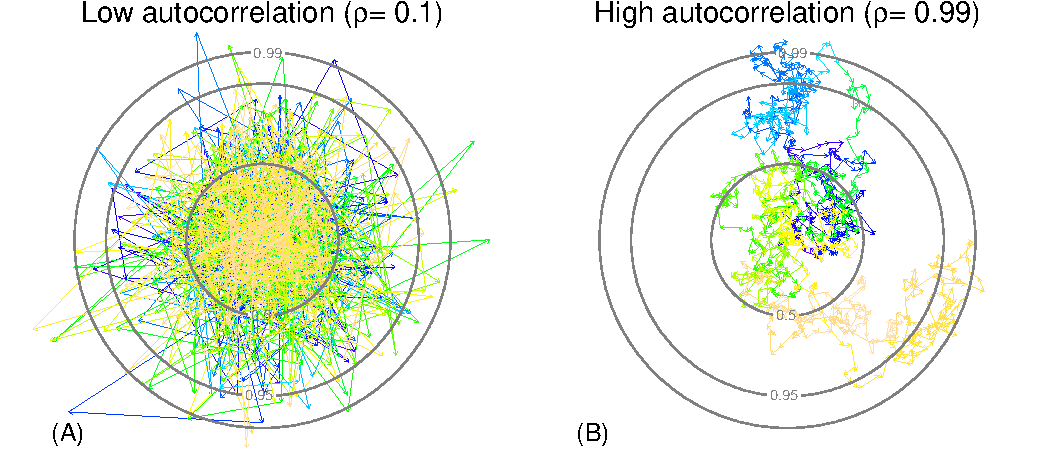
\includegraphics[width=0.9\textwidth]{figs/OU_low_high_contours} \\
  \caption{Two realizations of the Ornstein-Uhlenbeck process used to
    model animal movement. In both examples, the activity center and
    the variance parameter ($\sigma^2$) of the stationary distribution
    are the same. Consequently, isopleths of the long-term
    (stationary) utilization distributions are also the same. The
    difference lies in the correlation parameter ($\rho$) that
    controls the step lengths. Colors of the trajectories represent
    time.}   
  \label{fig:ou-concept}
\end{figure}


\clearpage


\begin{figure}[h!]
  \centering
  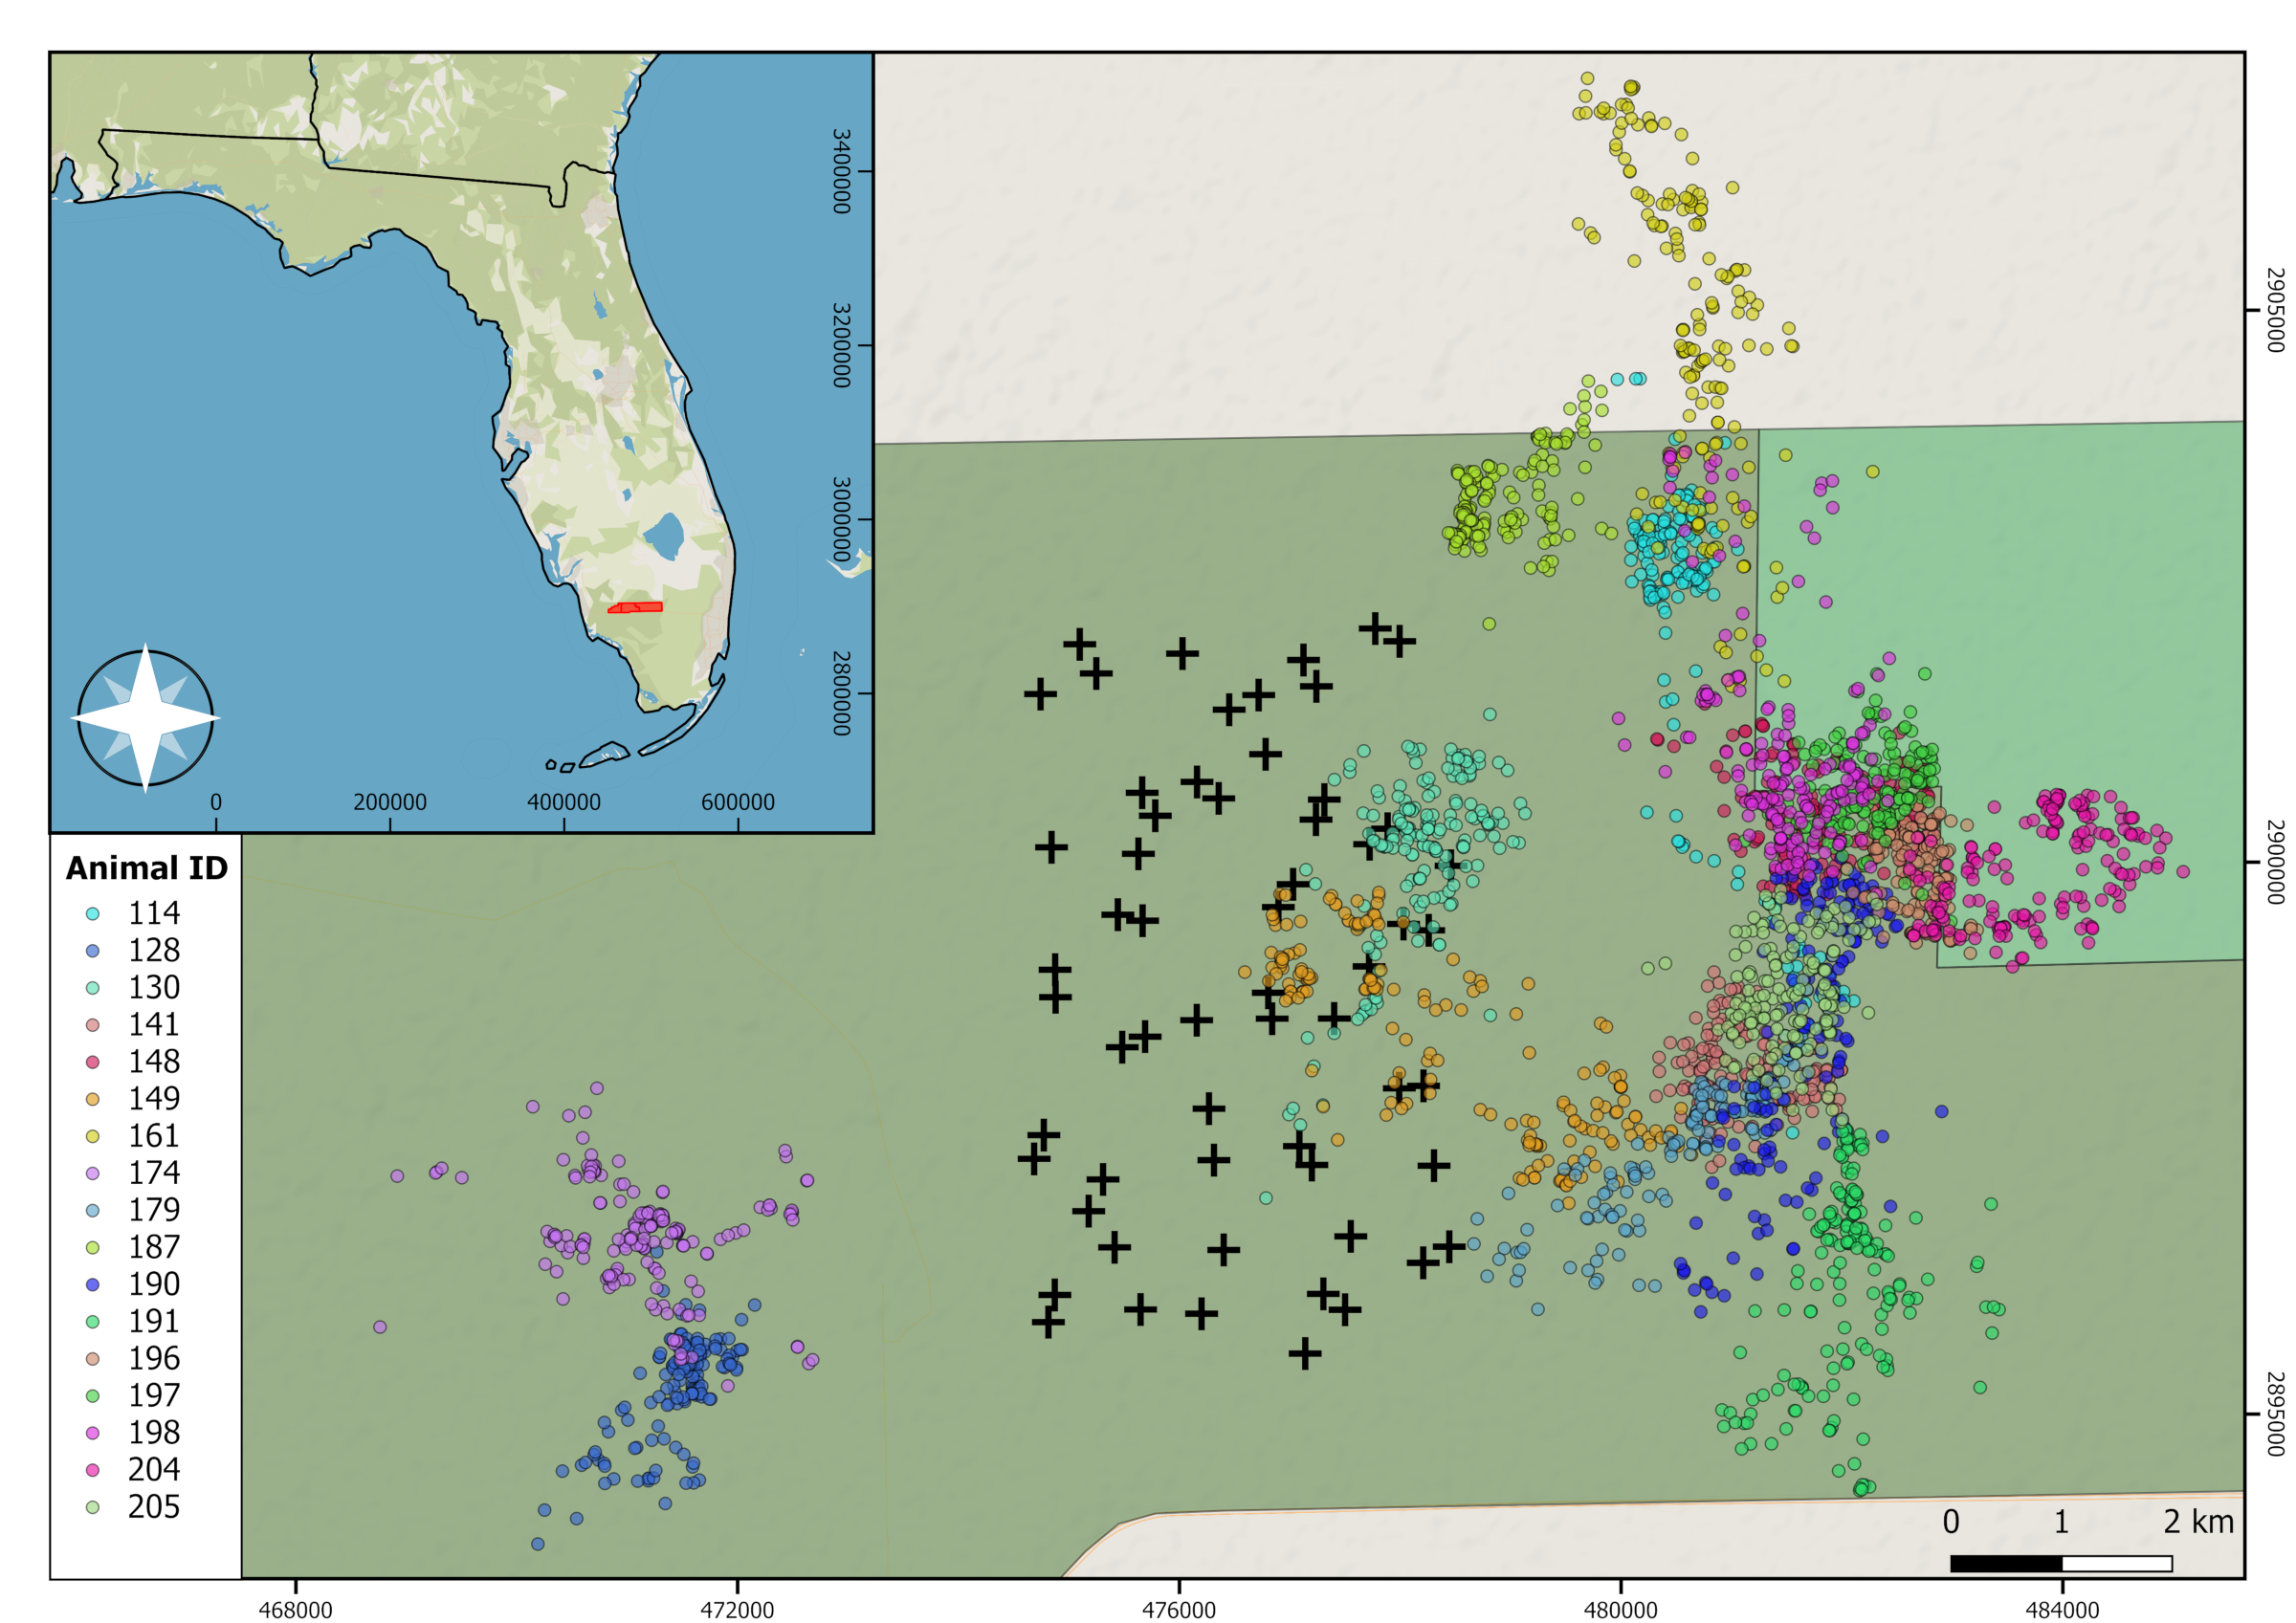
\includegraphics[width=\textwidth]{figs/StudyArea_6w_400dpi} \\
  \caption{Study area (red polygon in inset) in Big Cypress National Preserve, 
    Florida, USA. The 60 camera locations are shown as black
    crosses. Telemetry data from 17 male white-tailed deer in July
    2015 are shown as colored points.}
  \label{fig:study-area}
\end{figure}



\clearpage


\begin{figure}[h!]
  \centering
  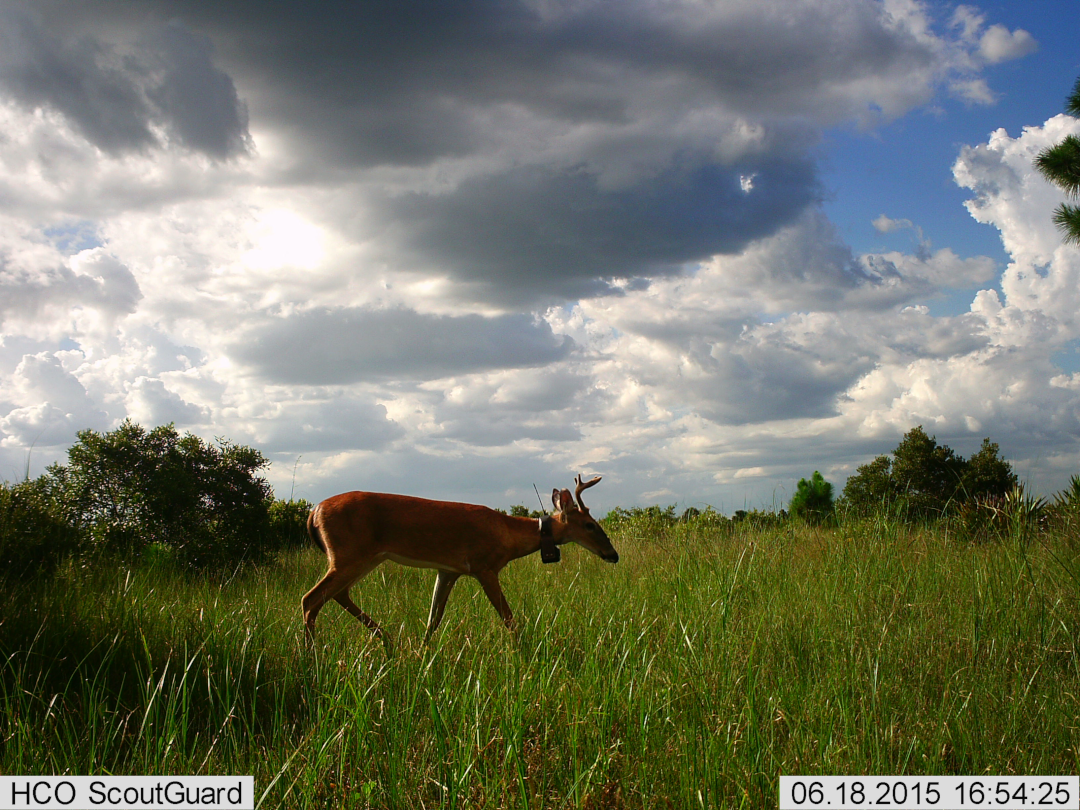
\includegraphics[width=0.49\textwidth, trim = 0mm 10mm 0mm 0mm, clip]{figs/buck_collar_6in} 
  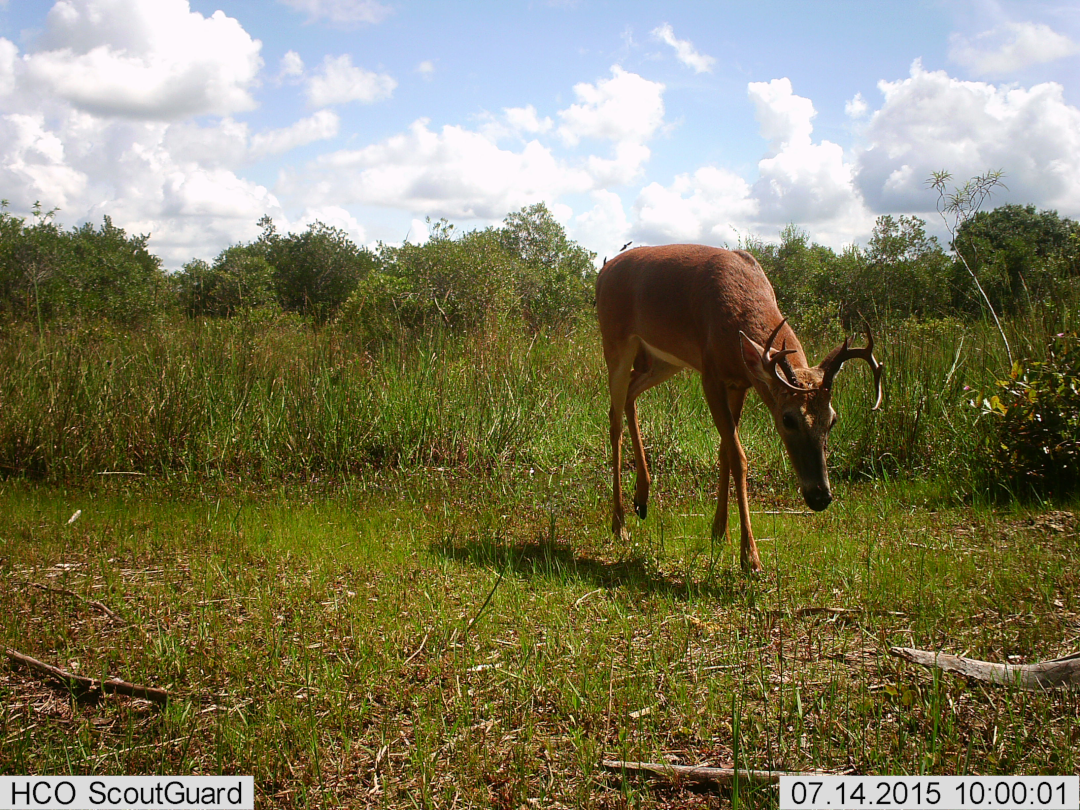
\includegraphics[width=0.49\textwidth, trim = 0mm 10mm 0mm 0mm, clip]{figs/buck_no_collar_6in} \\
  \caption{Two of the male white-tailed deer from South Florida, USA
    in July 2015. The individual on the left was captured and
    outfitted with a GPS transmitter. The individual on the right was
    uniquely identified based on antler morphology.} 
  \label{fig:bucks}
\end{figure}



\clearpage


\begin{figure}[h!]
  \centering
  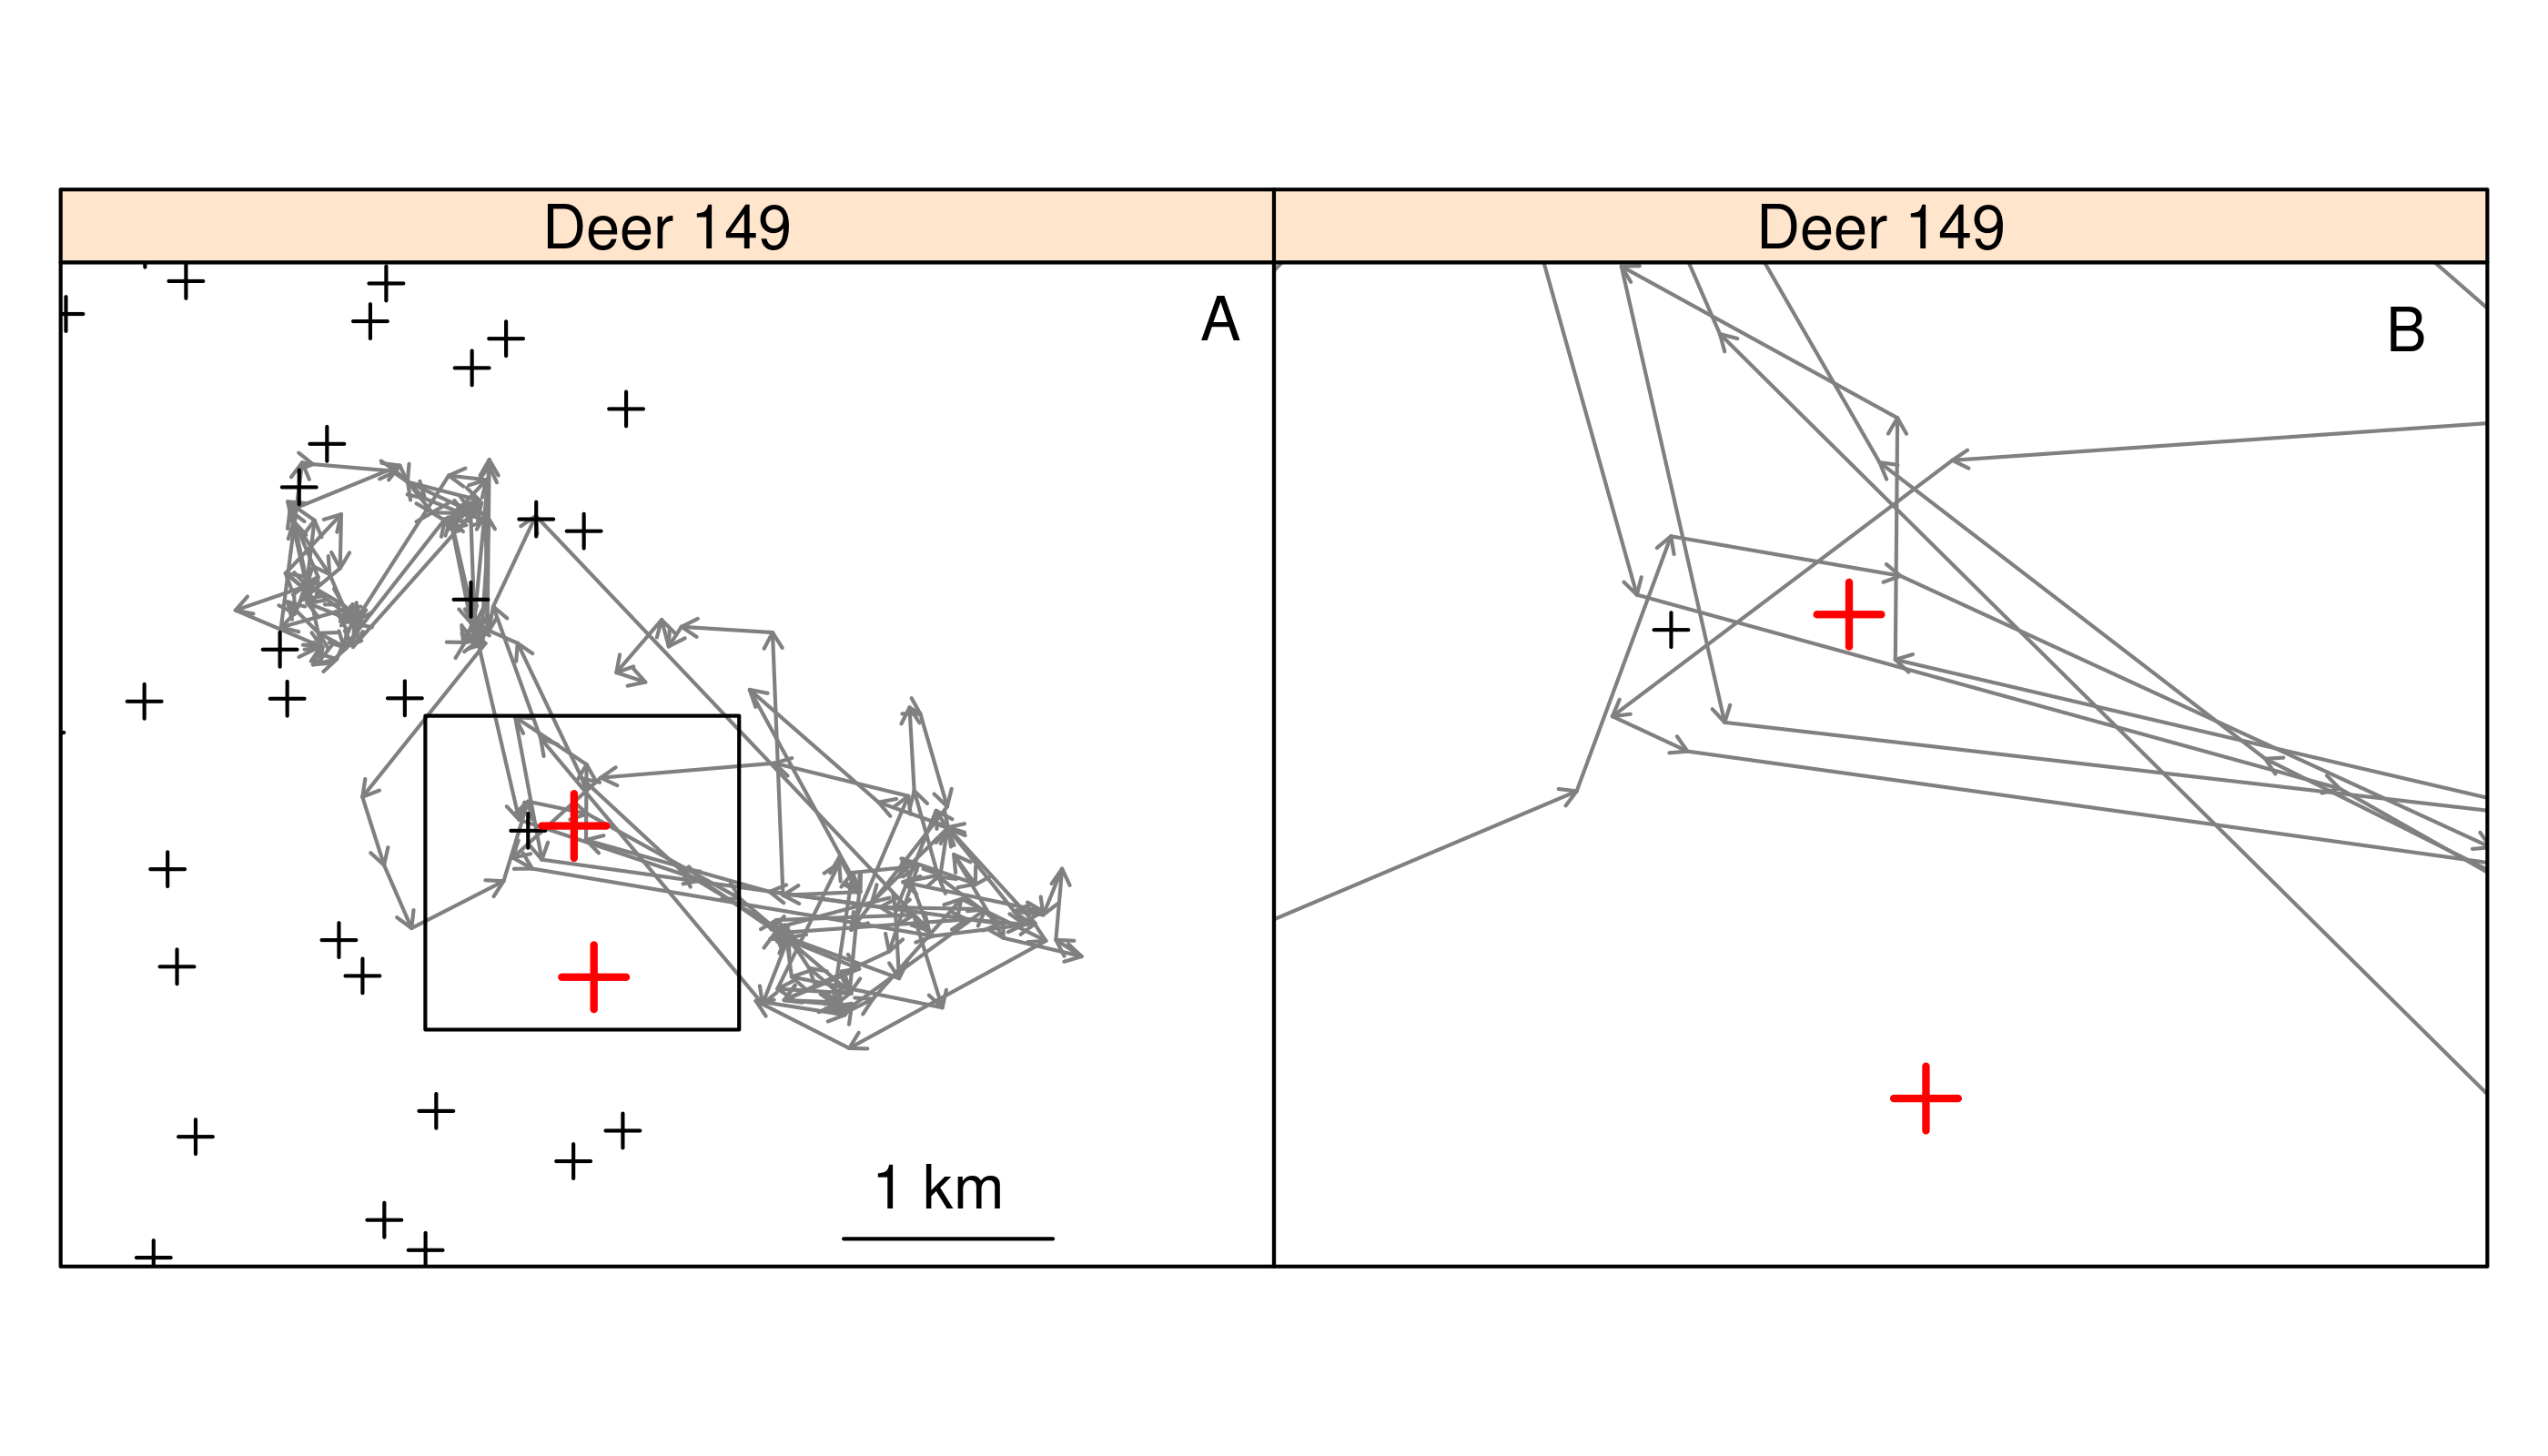
\includegraphics[width=0.9\textwidth]{figs/UD-path-149-zoom} \\
  \vspace{-1.1cm}
  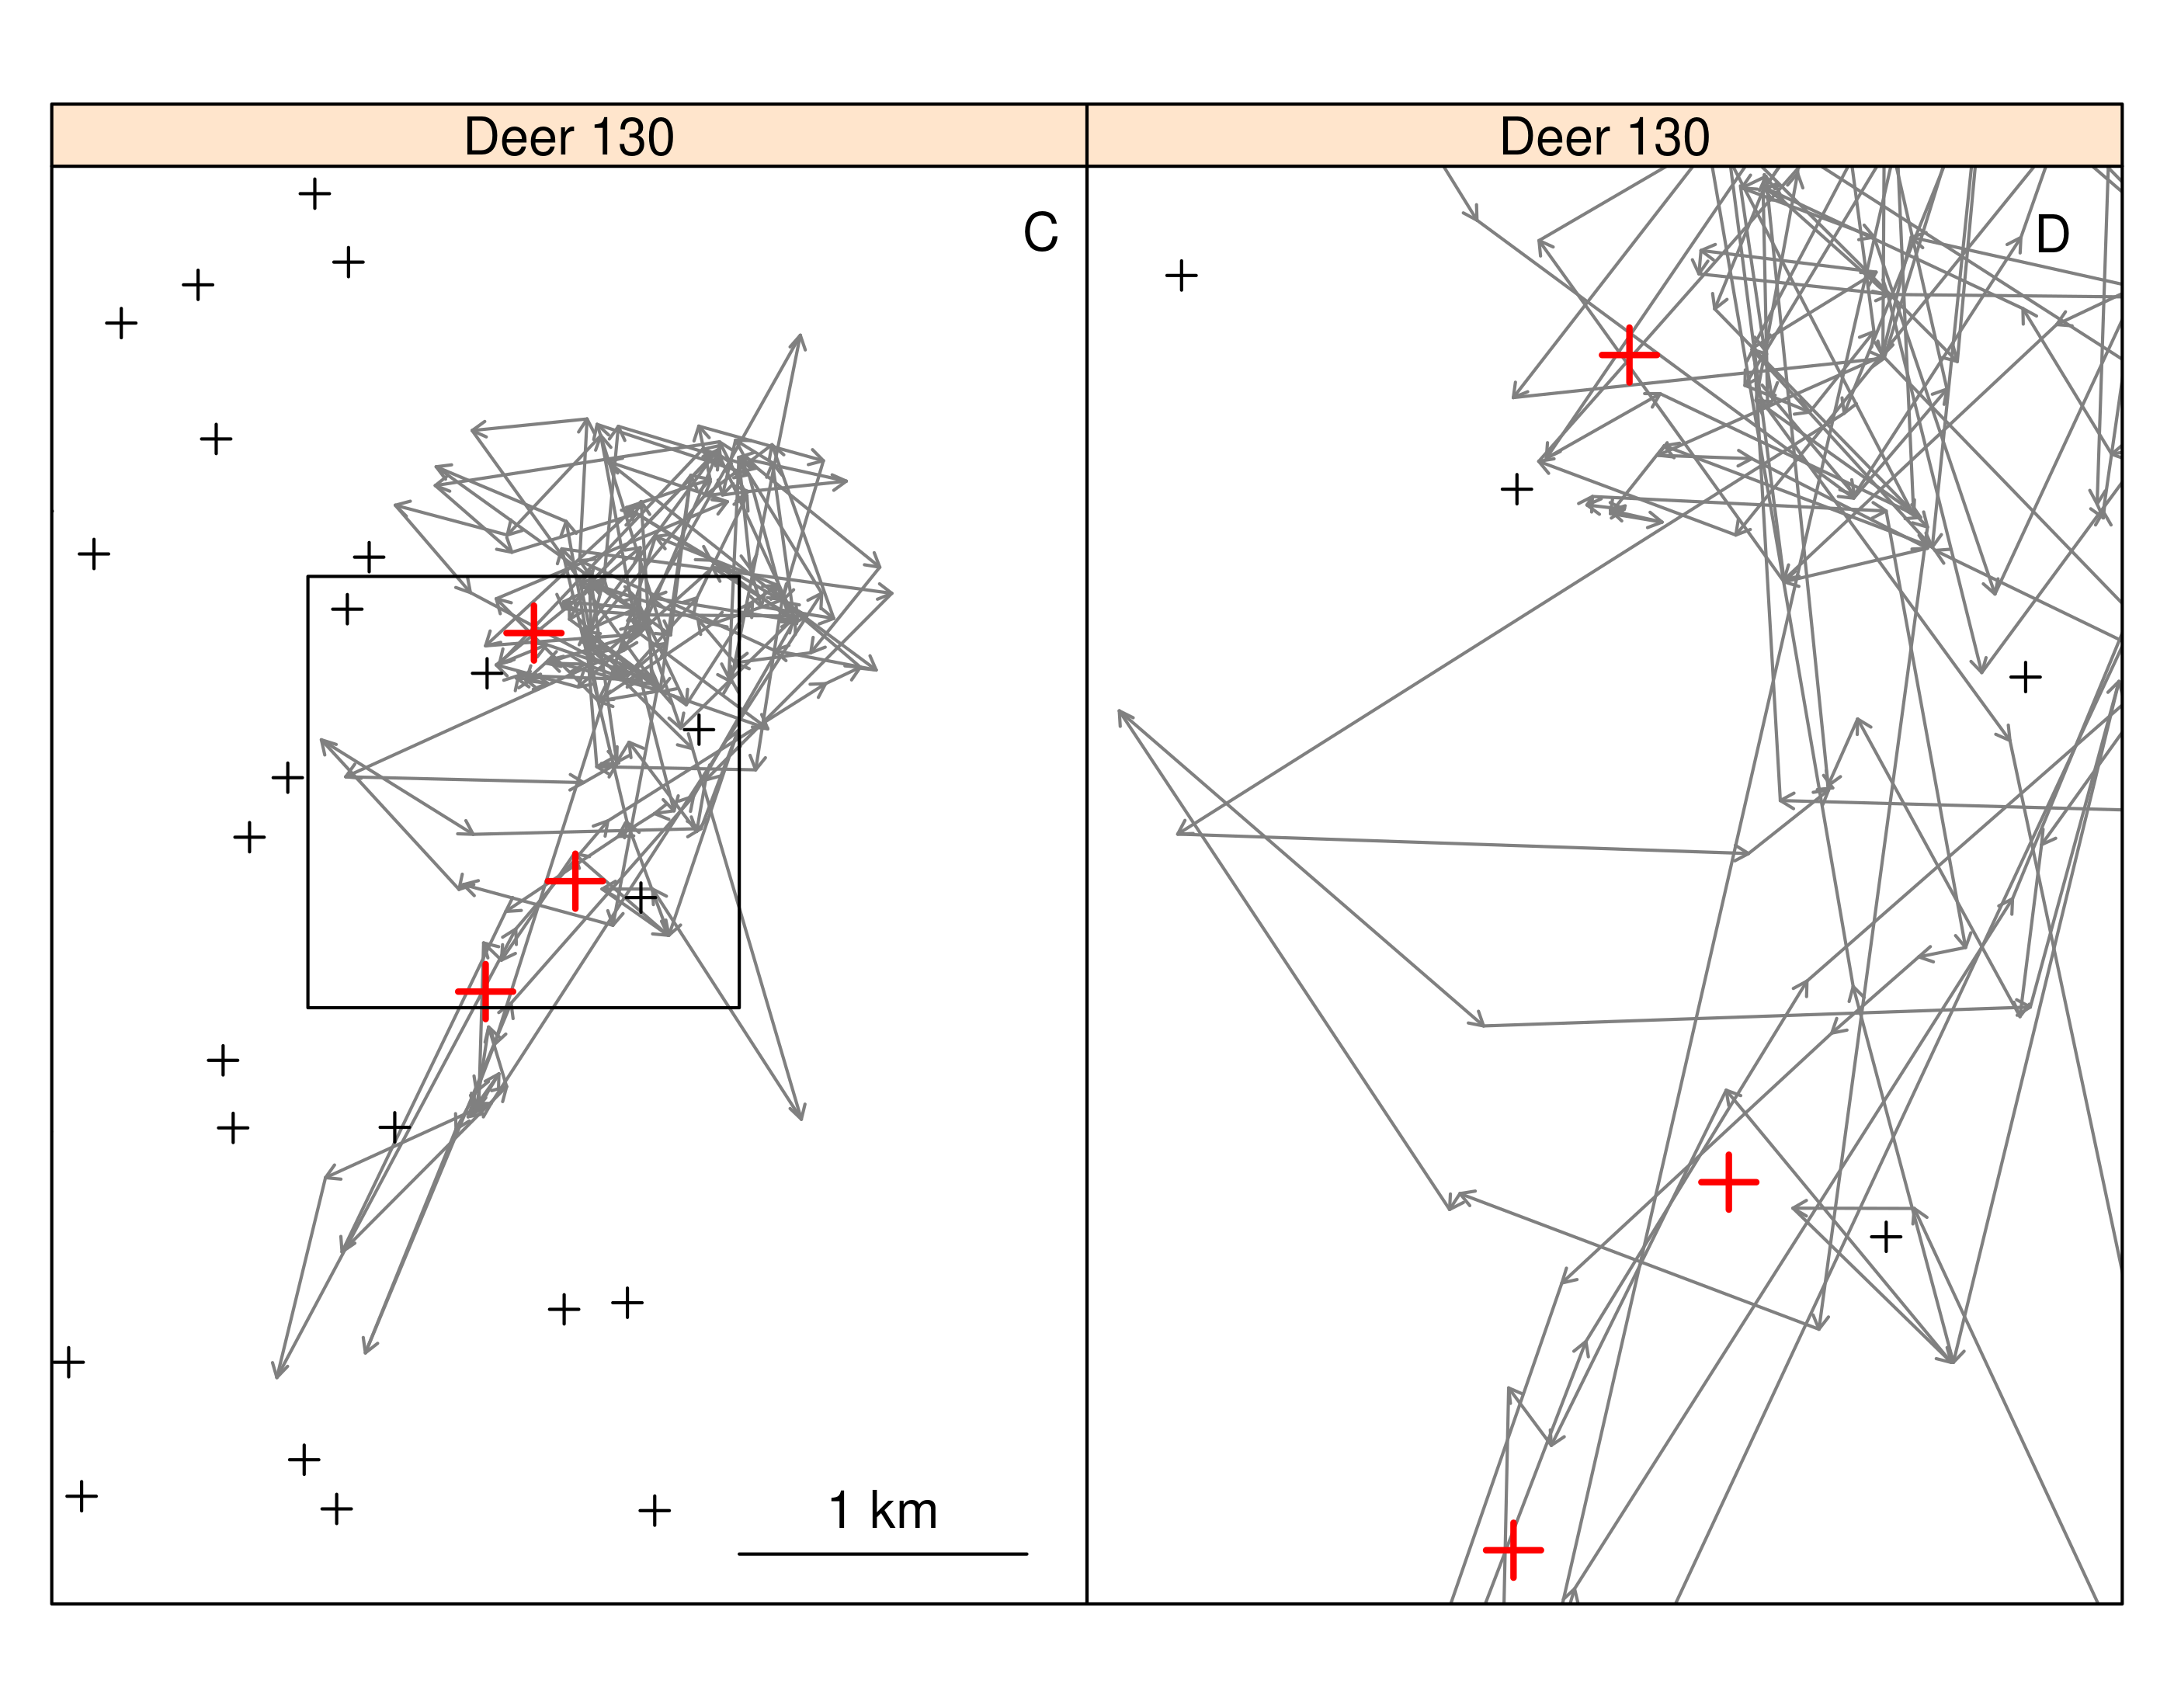
\includegraphics[width=0.9\textwidth]{figs/UD-path-130-zoom} \\
  \caption{Telemetry locations and detection events for the two
    white-tailed deer with GPS collars that were detected on cameras
    in South Florida, USA in July 2015. Panels A and C depict
    the observed movement paths. Panels B and D are zoomed in
    depictions of the rectangular regions on the left, showing how
    deer moved in relation to cameras where they were (red crosses)
    and were not (black crosses) detected. } 
  \label{fig:path-cam}
\end{figure}


\clearpage


\begin{figure}[h!]
  \centering
  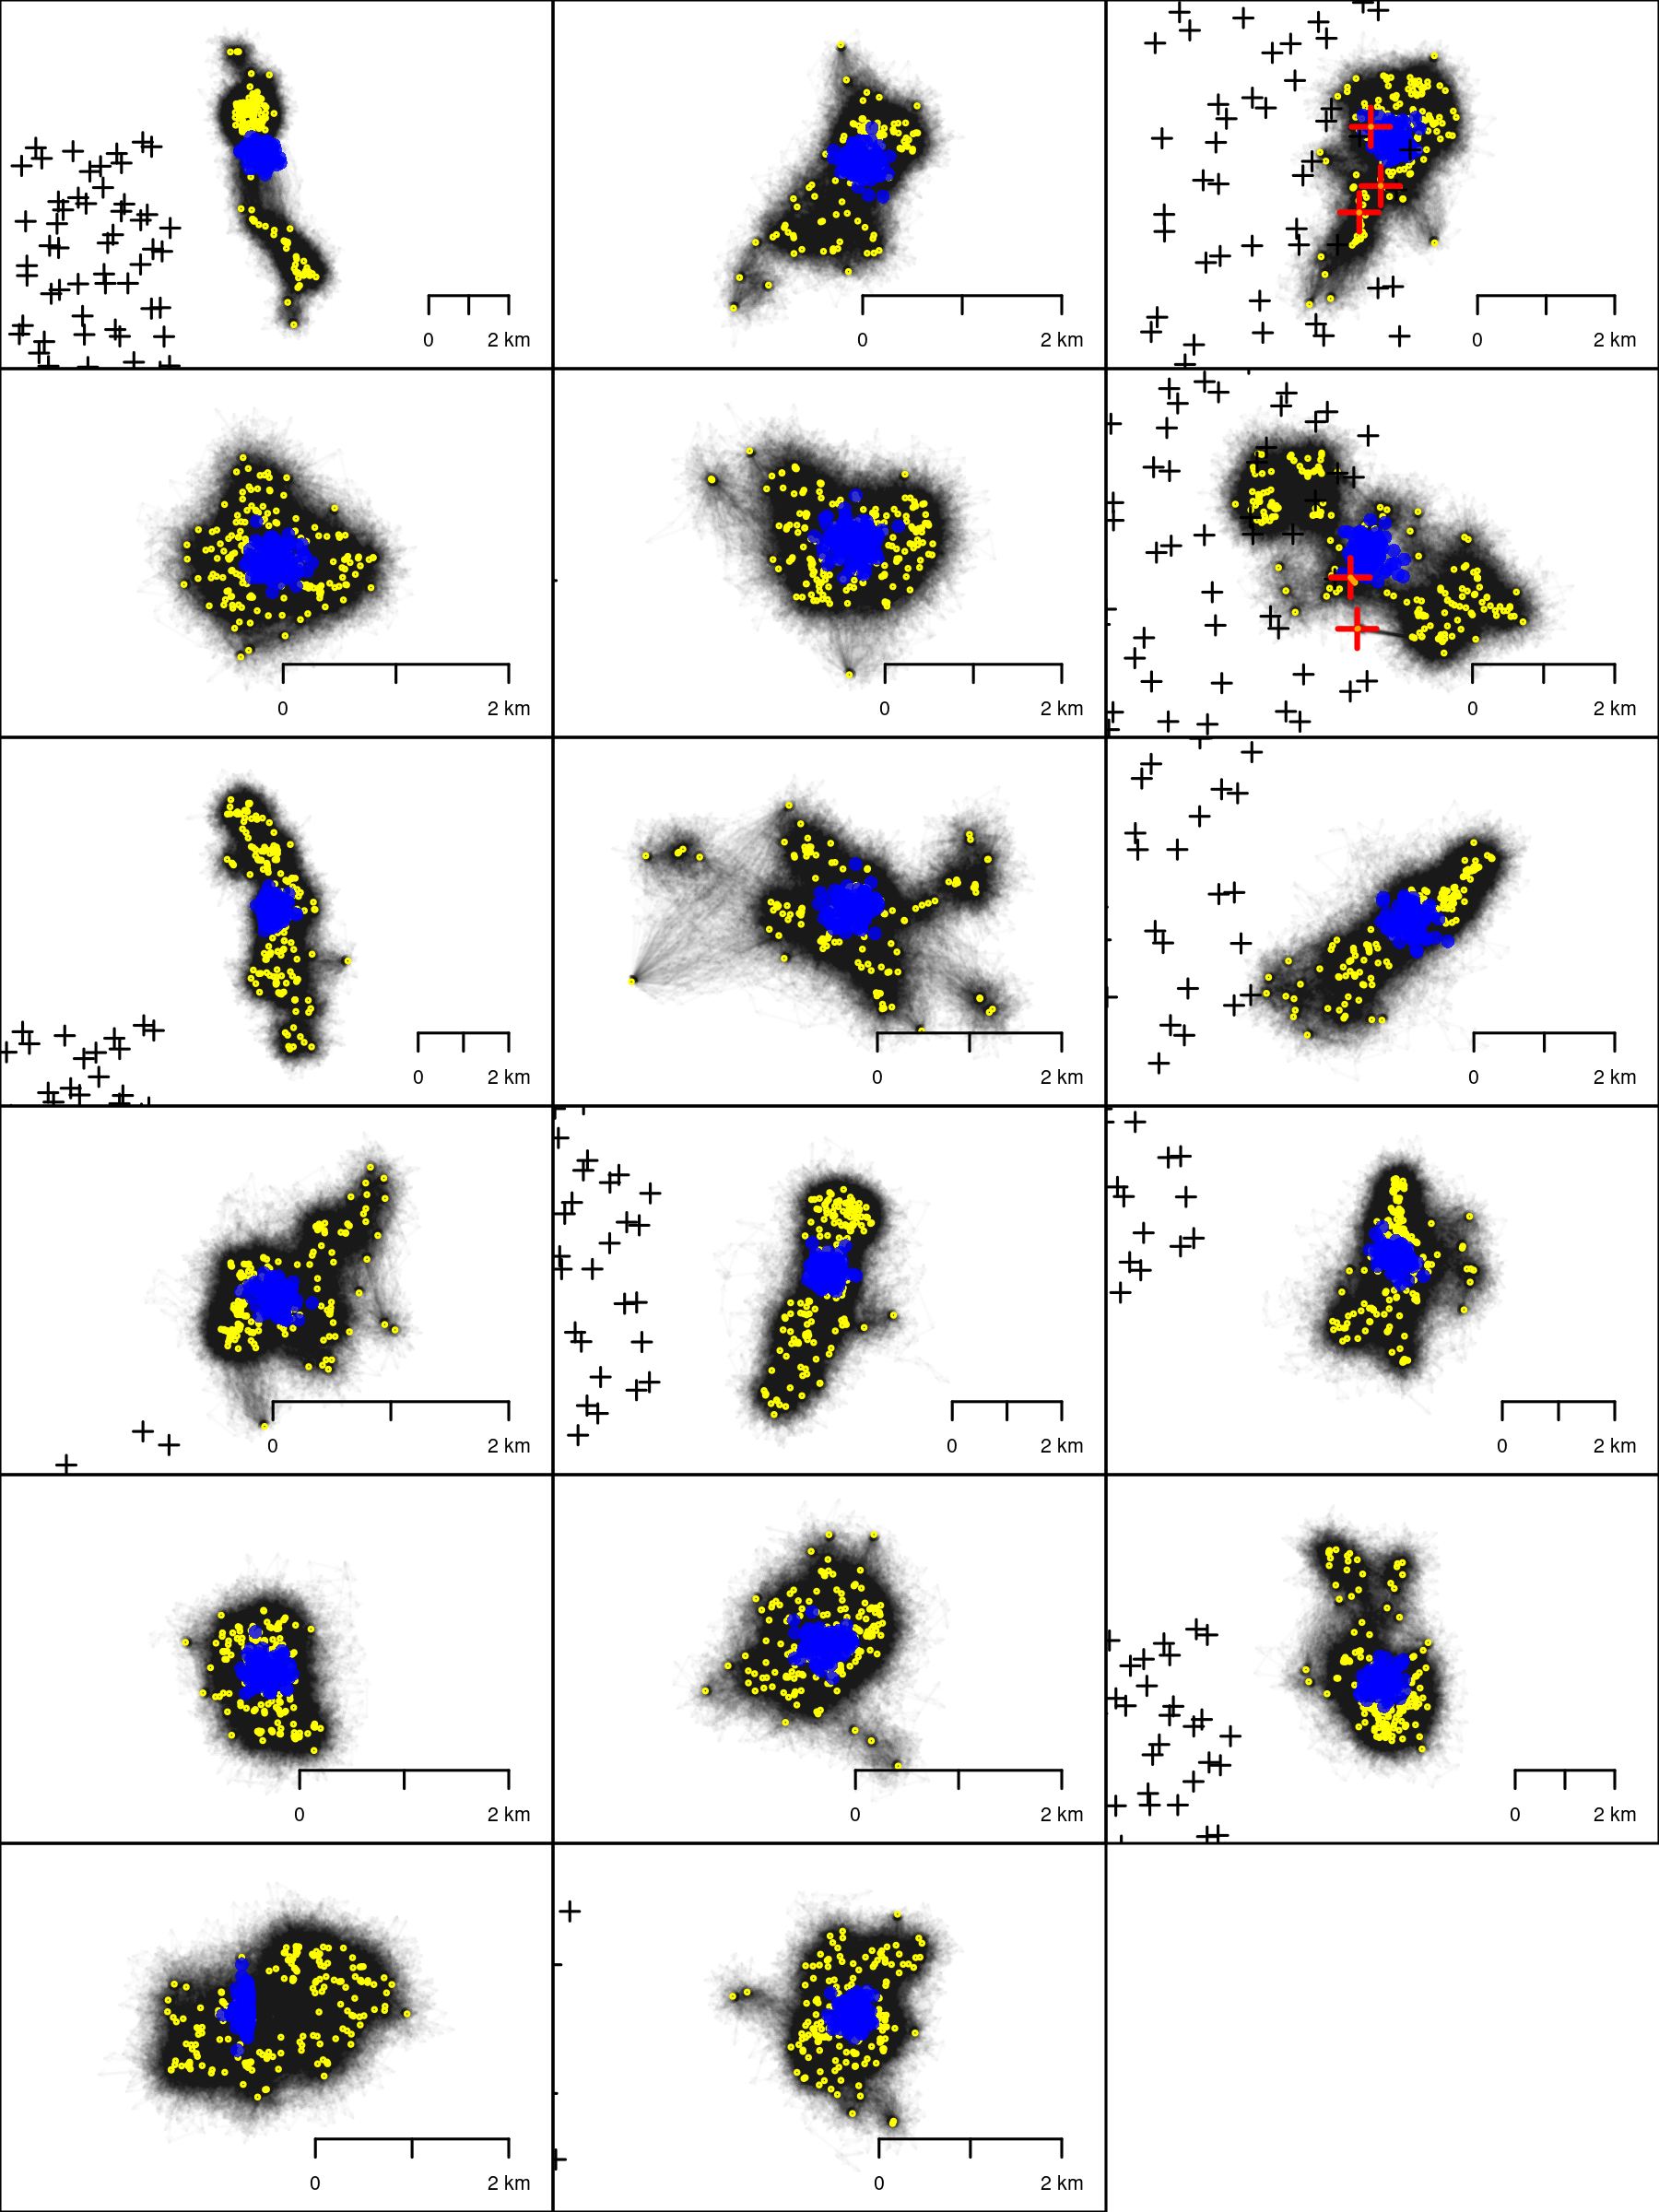
\includegraphics[width=0.8\textwidth]{figs/upost_panel} \\
  \caption{Telemetry locations (yellow points) with posterior samples
    of the Ornstein-Uhlenbeck movement paths (gray lines) and activity
    centers (blue points) for the 17 white-tailed deer with GPS
    telemetry data studied in South Florida, USA in July 2015. Camera
    locations are shown as crosses. Red crosses in the two panels at the
    upper-right indicate camera locations where a deer was detected. }  
  \label{fig:upost}
\end{figure}

\clearpage


\begin{figure}[h!]
  \centering
  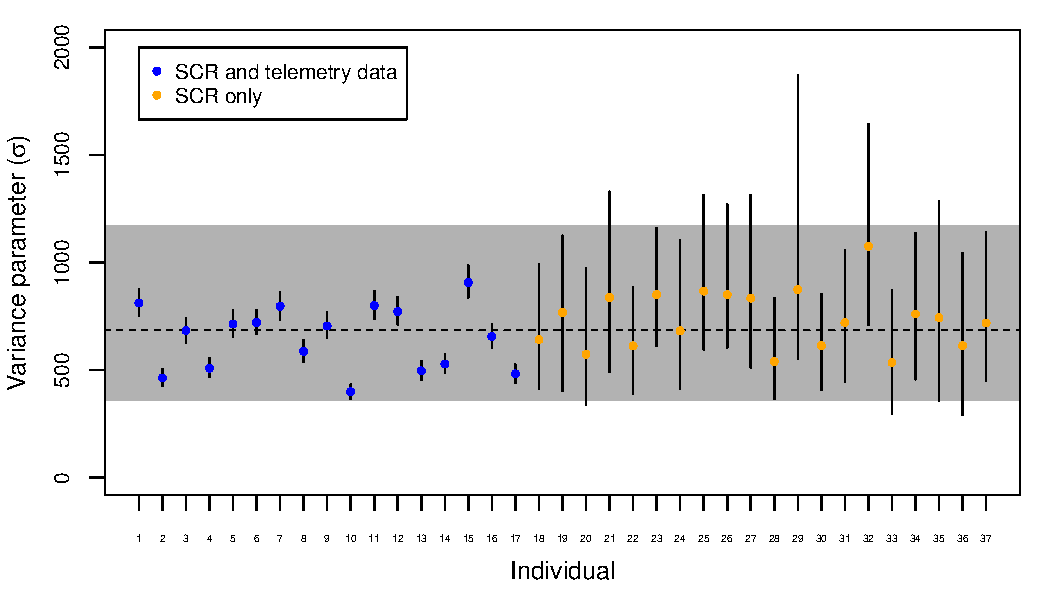
\includegraphics[width=\textwidth]{figs/sigma-re} \\
  \caption{Posterior means and 95\% CIs for the variance parameters
    ($\{\sigma_i\}$), which were modeled as log-normal random
    effects. As with standard SCR models, $\sigma$ is associated with
    the expected home range size, but in the joint SCR-movement model, it
    does not influence the detection function, which is controlled by
    $\lambda_0$ and $\sigma_{\mathrm  det}$. 
    The gray shaded region represents the 95\% CI for the random effects 
    distribution. The model was fitted to camera and telemetry data on
    male white-tailed deer studied in South Florida, USA in July 2015.} 
  \label{fig:sigma}
\end{figure}



\clearpage

\begin{figure}[h!]
  \centering
  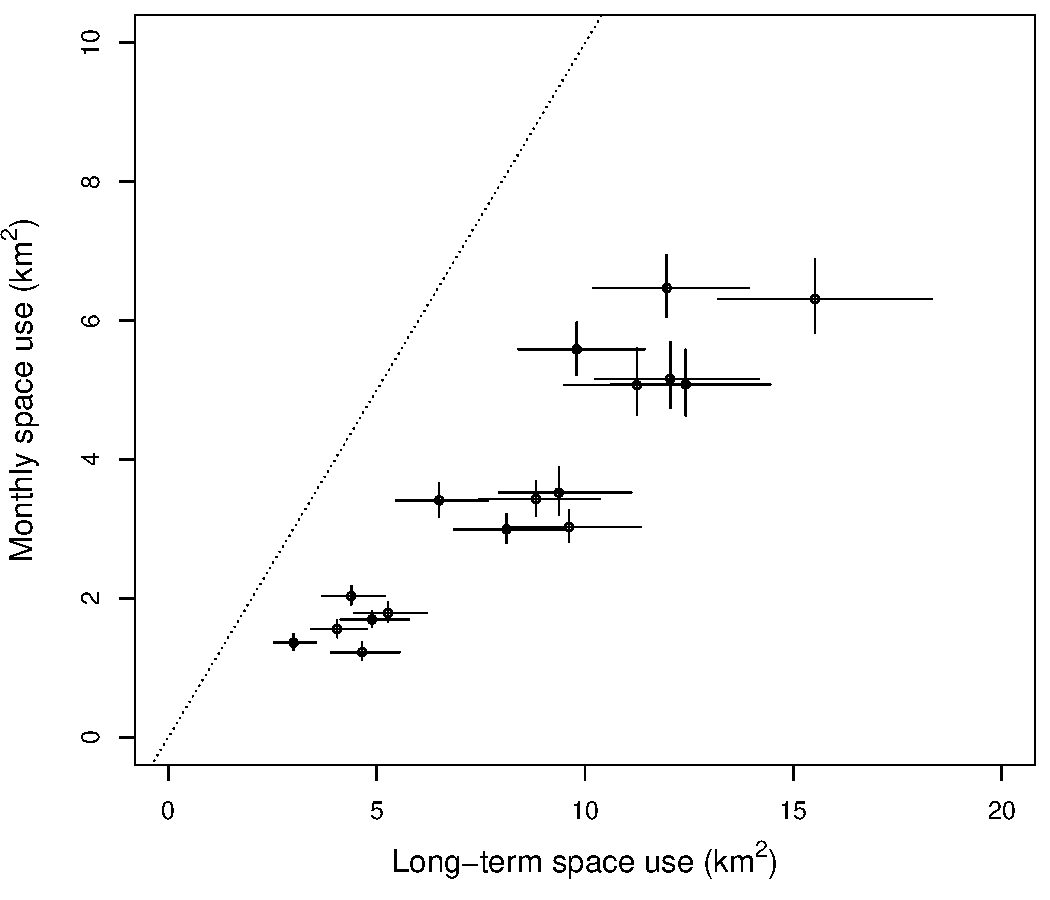
\includegraphics[width=0.8\textwidth]{figs/hr-e-r} \\
  \caption{Long-term and monthly space use based
    on 0.95 quantiles of the utilization distributions for the 17
    male white-tailed deer with GPS telemetry data from South Florida,
    USA in July 2015. The long-term estimates describe the
    area within which 95\% of locations from a Ornstein-Uhlenbeck
    movement process are {predicted} to be contained. The
    monthly estimates are from the utilization distributions
    associated with the partially-observed movement paths. } 
  \label{fig:hr}
\end{figure}



\clearpage


\begin{figure}[h!]
  \centering
  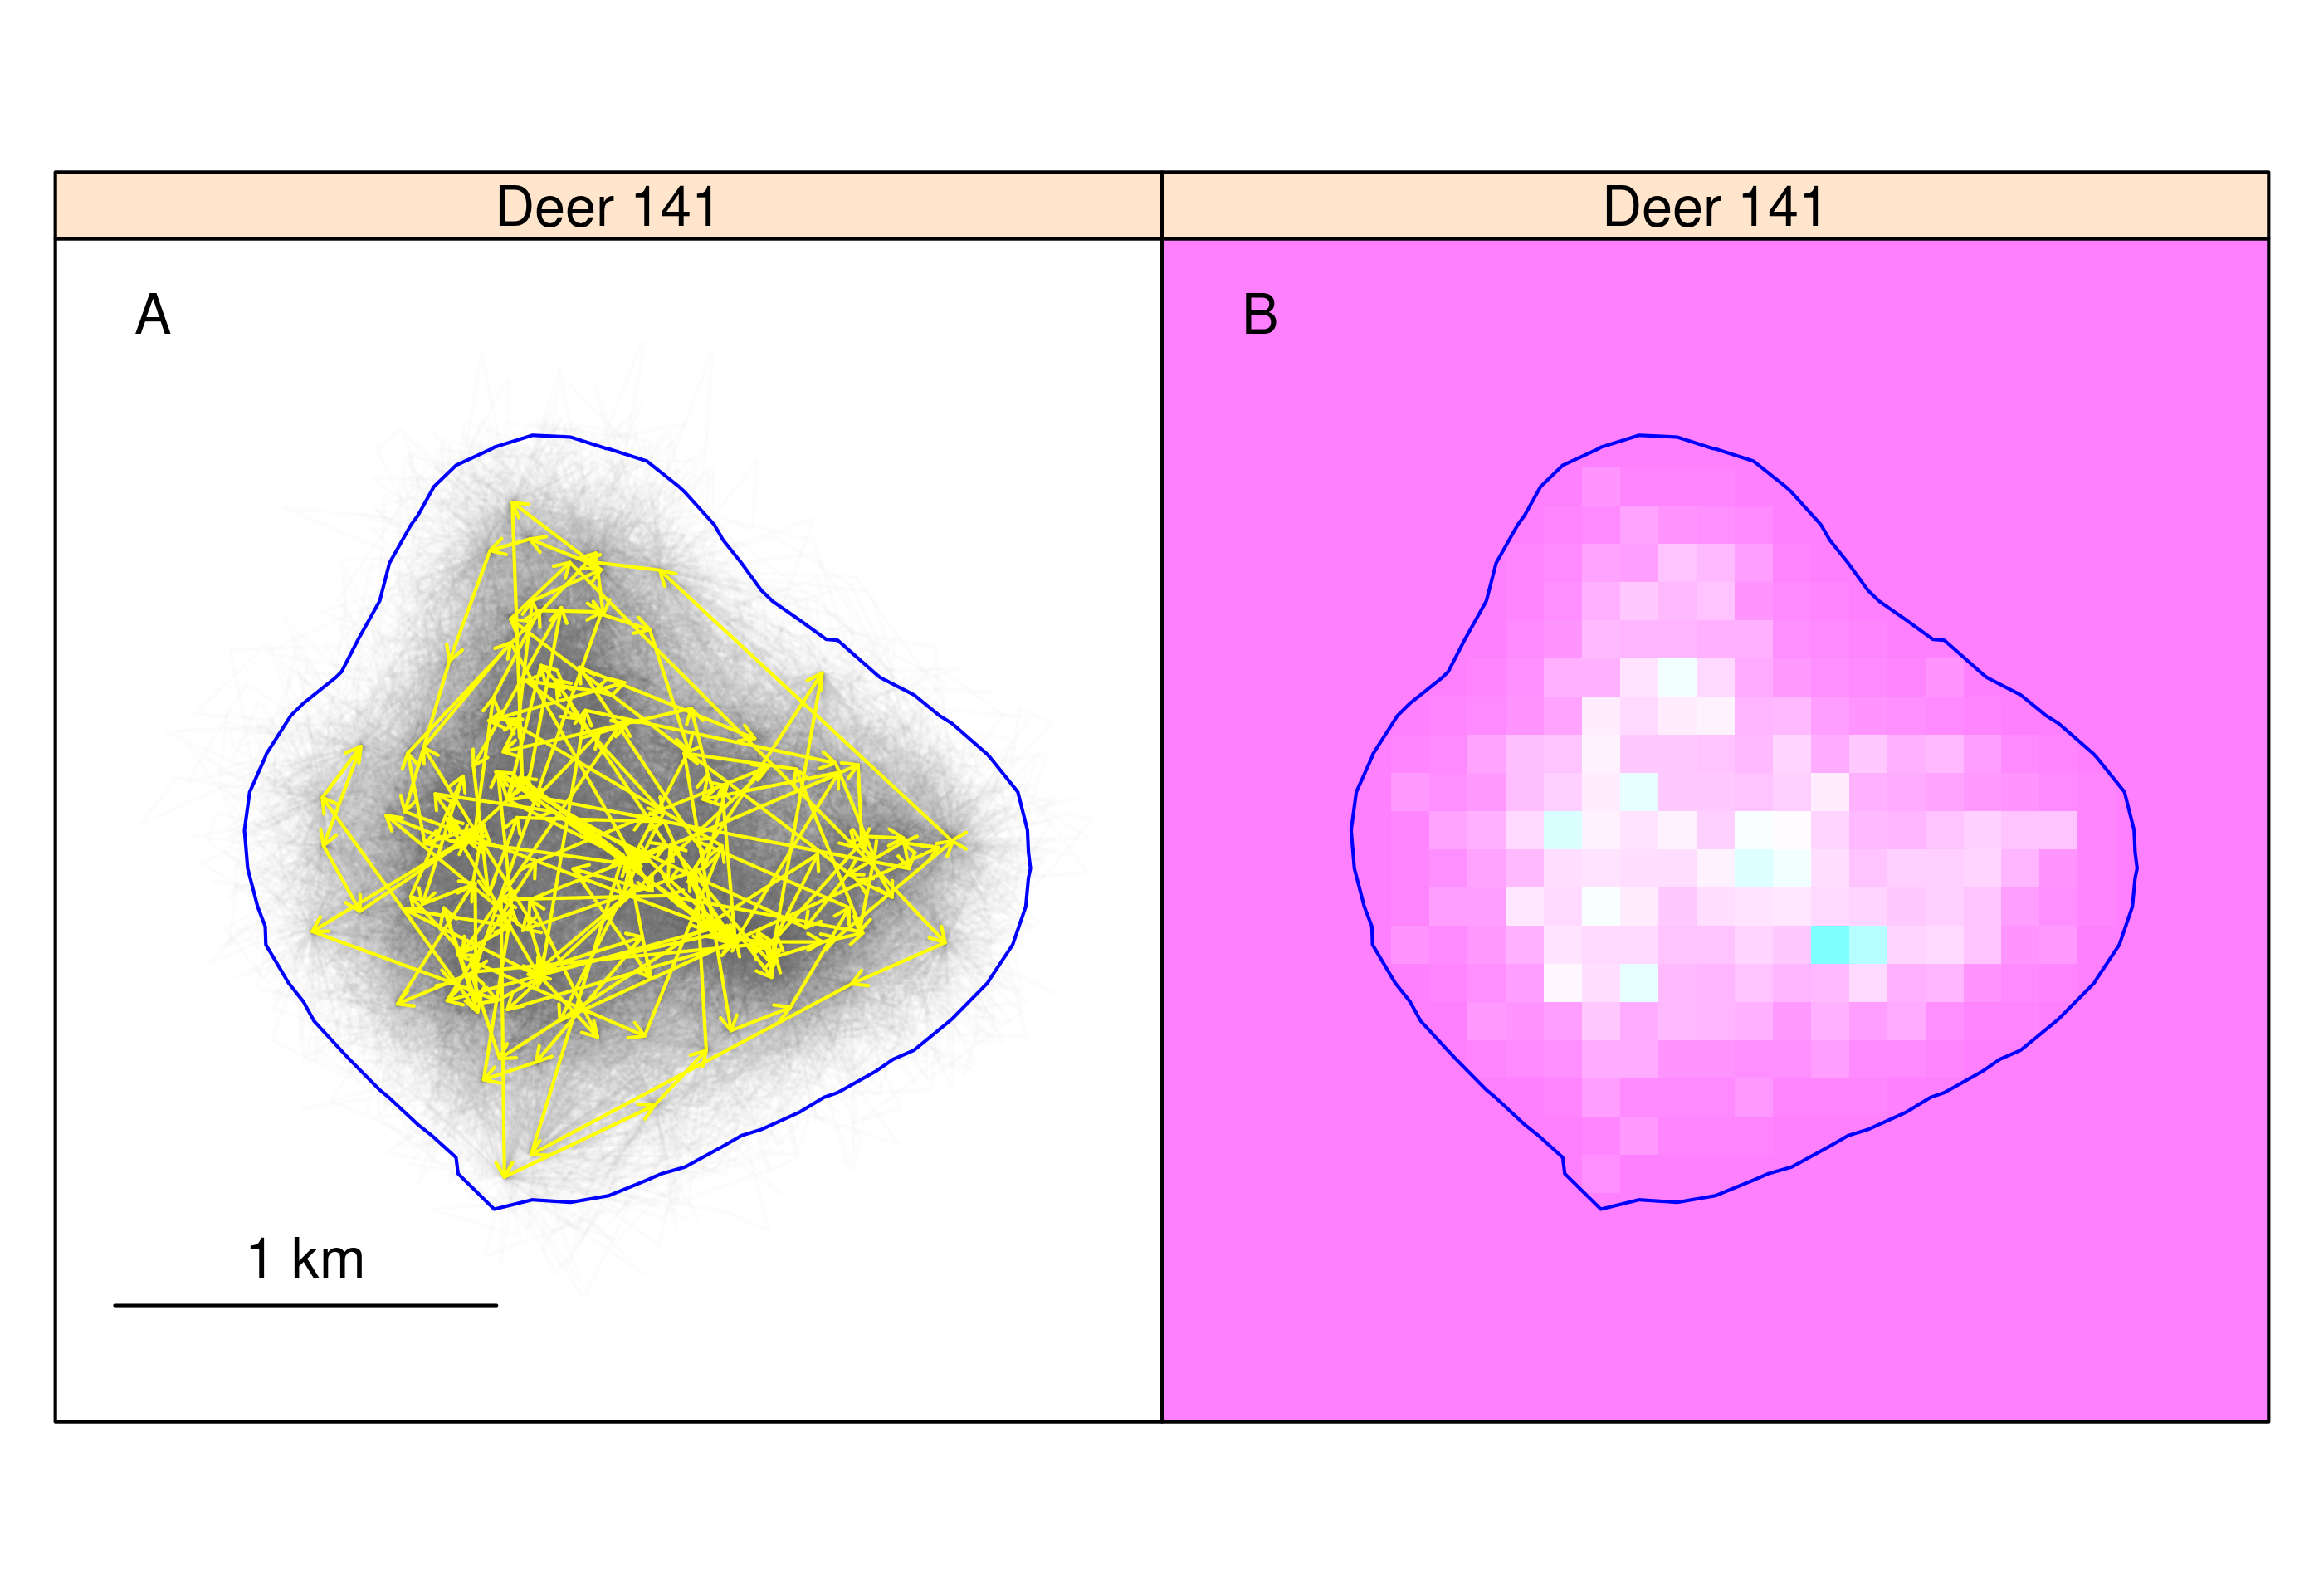
\includegraphics[width=0.7\textwidth]{figs/UD-path-141} \\
  \vspace{-0.8cm}
  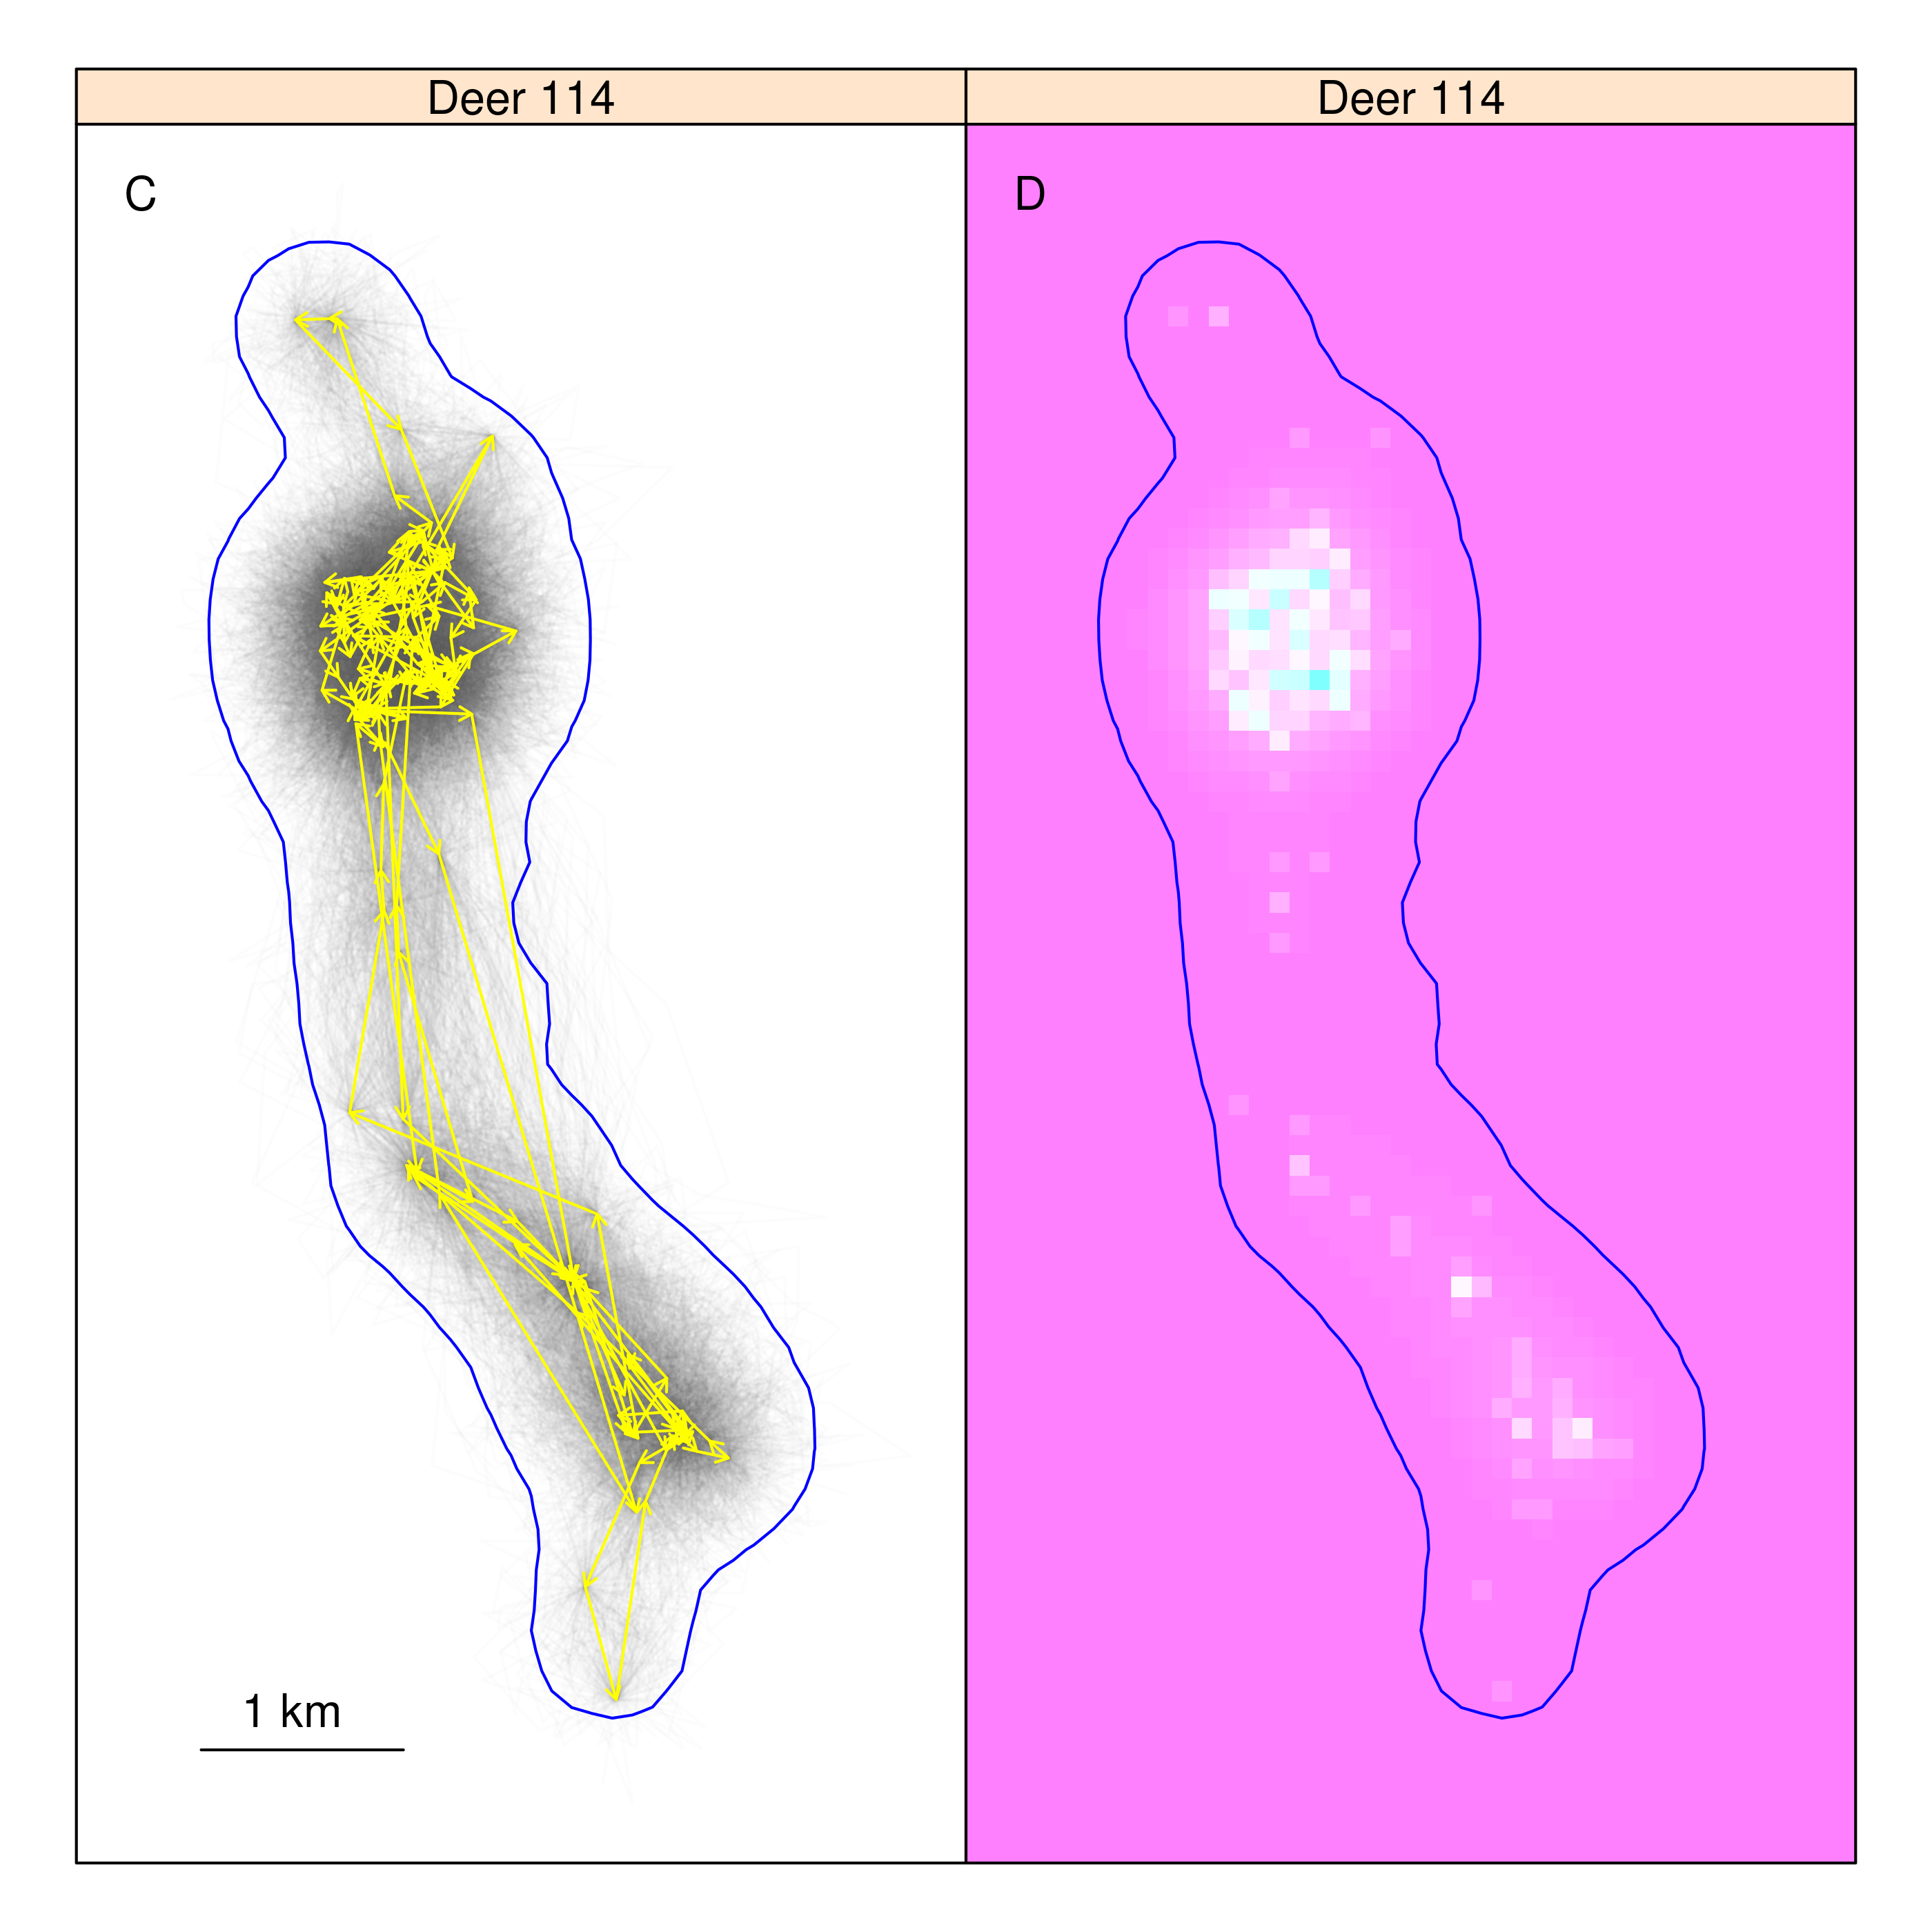
\includegraphics[width=0.72\textwidth]{figs/UD-path-114} \\
  \caption{Movement paths and utilization distributions for two of the
    17 male white-tailed deer with GPS collars. Panels A and C depict the observed
    movement paths in yellow, along with 100 posterior samples of the
    movement paths in gray. Panels B and D show the
    utilization distributions. The 99\% contours of the utilization
    distributions are shown in all panels. Data are from South
    Florida, USA in July 2015.} 
  \label{fig:path-ud}
\end{figure}





\end{document}
